% Created 2024-07-18 Thu 13:26
% Intended LaTeX compiler: xelatex
\documentclass[11pt]{article}
\usepackage{hyperref}
% wrong resolution of image
% https://tex.stackexchange.com/questions/21627/image-from-includegraphics-showing-in-wrong-image-size?rq=1

%%%%%%%%%%%%%%%%%%%%%%%%%%%%%%%%%%%%%%
%% TIPS                                 %%
%%%%%%%%%%%%%%%%%%%%%%%%%%%%%%%%%%%%%%
% \substack{a\\b} for multiple lines text
% \usepackage{expl3}
% \expandafter\def\csname ver@l3regex.sty\endcsname{}
% \usepackage{pkgloader}
\usepackage[utf8]{inputenc}

% nfss error
% \usepackage[B1,T1]{fontenc}
\usepackage{fontspec}

% \usepackage[Emoticons]{ucharclasses}
\newfontfamily\DejaSans{DejaVu Sans}
% \setDefaultTransitions{\DejaSans}{}

% pdfplots will load xolor automatically without option
\usepackage[dvipsnames]{xcolor}

%                                                             ┳┳┓   ┓
%                                                             ┃┃┃┏┓╋┣┓
%                                                             ┛ ┗┗┻┗┛┗
% \usepackage{amsmath} mathtools loads the amsmath
\usepackage{amsmath}
\usepackage{mathtools}

\usepackage{amsthm}
\usepackage{amsbsy}

%\usepackage{commath}

\usepackage{amssymb}

\usepackage{mathrsfs}
%\usepackage{mathabx}
\usepackage{stmaryrd}
\usepackage{empheq}

\usepackage{scalerel}
\usepackage{stackengine}
\usepackage{stackrel}



\usepackage{nicematrix}
\usepackage{tensor}
\usepackage{blkarray}
\usepackage{siunitx}
\usepackage[f]{esvect}

% centering \not on a letter
\usepackage{slashed}
\usepackage[makeroom]{cancel}

%\usepackage{merriweather}
\usepackage{unicode-math}
\setmainfont{TeX Gyre Pagella}
% \setmathfont{STIX}
%\setmathfont{texgyrepagella-math.otf}
%\setmathfont{Libertinus Math}
\setmathfont{Latin Modern Math}

 % \setmathfont[range={\smwhtdiamond,\enclosediamond,\varlrtriangle}]{Latin Modern Math}
\setmathfont[range={\rightrightarrows,\twoheadrightarrow,\leftrightsquigarrow,\triangledown,\vartriangle,\precneq,\succneq,\prec,\succ,\preceq,\succeq,\tieconcat}]{XITS Math}
 \setmathfont[range={\int,\setminus}]{Libertinus Math}
 % \setmathfont[range={\mathalpha}]{TeX Gyre Pagella Math}
%\setmathfont[range={\mitA,\mitB,\mitC,\mitD,\mitE,\mitF,\mitG,\mitH,\mitI,\mitJ,\mitK,\mitL,\mitM,\mitN,\mitO,\mitP,\mitQ,\mitR,\mitS,\mitT,\mitU,\mitV,\mitW,\mitX,\mitY,\mitZ,\mita,\mitb,\mitc,\mitd,\mite,\mitf,\mitg,\miti,\mitj,\mitk,\mitl,\mitm,\mitn,\mito,\mitp,\mitq,\mitr,\mits,\mitt,\mitu,\mitv,\mitw,\mitx,\mity,\mitz}]{TeX Gyre Pagella Math}
% unicode is not good at this!
%\let\nmodels\nvDash

 \usepackage{wasysym}

 % for wide hat
 \DeclareSymbolFont{yhlargesymbols}{OMX}{yhex}{m}{n} \DeclareMathAccent{\what}{\mathord}{yhlargesymbols}{"62}

%                                                               ┏┳┓•┓
%                                                                ┃ ┓┃┏┓
%                                                                ┻ ┗┛┗┗

\usepackage{pgfplots}
\pgfplotsset{compat=1.18}
\usepackage{tikz}
\usepackage{tikz-cd}
\tikzcdset{scale cd/.style={every label/.append style={scale=#1},
    cells={nodes={scale=#1}}}}
% TODO: discard qtree and use forest
% \usepackage{tikz-qtree}
\usepackage{forest}

\usetikzlibrary{arrows,positioning,calc,fadings,decorations,matrix,decorations,shapes.misc}
%setting from geogebra
\definecolor{ccqqqq}{rgb}{0.8,0,0}

%                                                          ┳┳┓•    ┓┓
%                                                          ┃┃┃┓┏┏┏┓┃┃┏┓┏┓┏┓┏┓┓┏┏
%                                                          ┛ ┗┗┛┗┗ ┗┗┗┻┛┗┗ ┗┛┗┻┛
%\usepackage{twemojis}
\usepackage[most]{tcolorbox}
\usepackage{threeparttable}
\usepackage{tabularx}

\usepackage{enumitem}
\usepackage[indLines=false]{algpseudocodex}
\usepackage[]{algorithm2e}
% \SetKwComment{Comment}{/* }{ */}
% \algrenewcommand\algorithmicrequire{\textbf{Input:}}
% \algrenewcommand\algorithmicensure{\textbf{Output:}}
% wrong with preview
\usepackage{subcaption}
\usepackage{caption}
% {\aunclfamily\Huge}
\usepackage{auncial}

\usepackage{float}

\usepackage{fancyhdr}

\usepackage{ifthen}
\usepackage{xargs}

\definecolor{mintedbg}{rgb}{0.99,0.99,0.99}
\usepackage[cachedir=\detokenize{~/miscellaneous/trash}]{minted}
\setminted{breaklines,
  mathescape,
  bgcolor=mintedbg,
  fontsize=\footnotesize,
  frame=single,
  linenos}
\usemintedstyle{xcode}
\usepackage{tcolorbox}
\usepackage{etoolbox}



\usepackage{imakeidx}
\usepackage{hyperref}
\usepackage{soul}
\usepackage{framed}

% don't use this for preview
%\usepackage[margin=1.5in]{geometry}
% \usepackage{geometry}
% \geometry{legalpaper, landscape, margin=1in}
\usepackage[font=itshape]{quoting}

%\LoadPackagesNow
%\usepackage[xetex]{preview}
%%%%%%%%%%%%%%%%%%%%%%%%%%%%%%%%%%%%%%%
%% USEPACKAGES end                       %%
%%%%%%%%%%%%%%%%%%%%%%%%%%%%%%%%%%%%%%%

%%%%%%%%%%%%%%%%%%%%%%%%%%%%%%%%%%%%%%%
%% Algorithm environment
%%%%%%%%%%%%%%%%%%%%%%%%%%%%%%%%%%%%%%%
\SetKwIF{Recv}{}{}{upon receiving}{do}{}{}{}
\SetKwBlock{Init}{initially do}{}
\SetKwProg{Function}{Function}{:}{}

% https://github.com/chrmatt/algpseudocodex/issues/3
\algnewcommand\algorithmicswitch{\textbf{switch}}%
\algnewcommand\algorithmiccase{\textbf{case}}
\algnewcommand\algorithmicof{\textbf{of}}
\algnewcommand\algorithmicotherwise{\texttt{otherwise} $\Rightarrow$}

\makeatletter
\algdef{SE}[SWITCH]{Switch}{EndSwitch}[1]{\algpx@startIndent\algpx@startCodeCommand\algorithmicswitch\ #1\ \algorithmicdo}{\algpx@endIndent\algpx@startCodeCommand\algorithmicend\ \algorithmicswitch}%
\algdef{SE}[CASE]{Case}{EndCase}[1]{\algpx@startIndent\algpx@startCodeCommand\algorithmiccase\ #1}{\algpx@endIndent\algpx@startCodeCommand\algorithmicend\ \algorithmiccase}%
\algdef{SE}[CASEOF]{CaseOf}{EndCaseOf}[1]{\algpx@startIndent\algpx@startCodeCommand\algorithmiccase\ #1 \algorithmicof}{\algpx@endIndent\algpx@startCodeCommand\algorithmicend\ \algorithmiccase}
\algdef{SE}[OTHERWISE]{Otherwise}{EndOtherwise}[0]{\algpx@startIndent\algpx@startCodeCommand\algorithmicotherwise}{\algpx@endIndent\algpx@startCodeCommand\algorithmicend\ \algorithmicotherwise}
\ifbool{algpx@noEnd}{%
  \algtext*{EndSwitch}%
  \algtext*{EndCase}%
  \algtext*{EndCaseOf}
  \algtext*{EndOtherwise}
  %
  % end indent line after (not before), to get correct y position for multiline text in last command
  \apptocmd{\EndSwitch}{\algpx@endIndent}{}{}%
  \apptocmd{\EndCase}{\algpx@endIndent}{}{}%
  \apptocmd{\EndCaseOf}{\algpx@endIndent}{}{}
  \apptocmd{\EndOtherwise}{\algpx@endIndent}{}{}
}{}%

\pretocmd{\Switch}{\algpx@endCodeCommand}{}{}
\pretocmd{\Case}{\algpx@endCodeCommand}{}{}
\pretocmd{\CaseOf}{\algpx@endCodeCommand}{}{}
\pretocmd{\Otherwise}{\algpx@endCodeCommand}{}{}

% for end commands that may not be printed, tell endCodeCommand whether we are using noEnd
\ifbool{algpx@noEnd}{%
  \pretocmd{\EndSwitch}{\algpx@endCodeCommand[1]}{}{}%
  \pretocmd{\EndCase}{\algpx@endCodeCommand[1]}{}{}
  \pretocmd{\EndCaseOf}{\algpx@endCodeCommand[1]}{}{}%
  \pretocmd{\EndOtherwise}{\algpx@endCodeCommand[1]}{}{}
}{%
  \pretocmd{\EndSwitch}{\algpx@endCodeCommand[0]}{}{}%
  \pretocmd{\EndCase}{\algpx@endCodeCommand[0]}{}{}%
  \pretocmd{\EndCaseOf}{\algpx@endCodeCommand[0]}{}{}
  \pretocmd{\EndOtherwise}{\algpx@endCodeCommand[0]}{}{}
}%
\makeatother
% % For algpseudocode
% \algnewcommand\algorithmicswitch{\textbf{switch}}
% \algnewcommand\algorithmiccase{\textbf{case}}
% \algnewcommand\algorithmiccaseof{\textbf{case}}
% \algnewcommand\algorithmicof{\textbf{of}}
% % New "environments"
% \algdef{SE}[SWITCH]{Switch}{EndSwitch}[1]{\algorithmicswitch\ #1\ \algorithmicdo}{\algorithmicend\ \algorithmicswitch}%
% \algdef{SE}[CASE]{Case}{EndCase}[1]{\algorithmiccase\ #1}{\algorithmicend\ \algorithmiccase}%
% \algtext*{EndSwitch}%
% \algtext*{EndCase}
% \algdef{SE}[CASEOF]{CaseOf}{EndCaseOf}[1]{\algorithmiccaseof\ #1 \algorithmicof}{\algorithmicend\ \algorithmiccaseof}
% \algtext*{EndCaseOf}



%\pdfcompresslevel0

% quoting from
% https://tex.stackexchange.com/questions/391726/the-quotation-environment
\NewDocumentCommand{\bywhom}{m}{% the Bourbaki trick
  {\nobreak\hfill\penalty50\hskip1em\null\nobreak
   \hfill\mbox{\normalfont(#1)}%
   \parfillskip=0pt \finalhyphendemerits=0 \par}%
}

\NewDocumentEnvironment{pquotation}{m}
  {\begin{quoting}[
     indentfirst=true,
     leftmargin=\parindent,
     rightmargin=\parindent]\itshape}
  {\bywhom{#1}\end{quoting}}

\indexsetup{othercode=\small}
\makeindex[columns=2,options={-s /media/wu/file/stuuudy/notes/index_style.ist},intoc]
\makeatletter
\def\@idxitem{\par\hangindent 0pt}
\makeatother


% \newcounter{dummy} \numberwithin{dummy}{section}
\newtheorem{dummy}{dummy}[section]
\theoremstyle{definition}
\newtheorem{definition}[dummy]{Definition}
\theoremstyle{plain}
\newtheorem{corollary}[dummy]{Corollary}
\newtheorem{lemma}[dummy]{Lemma}
\newtheorem{proposition}[dummy]{Proposition}
\newtheorem{theorem}[dummy]{Theorem}
\newtheorem{notation}[dummy]{Notation}
\newtheorem{conjecture}[dummy]{Conjecture}
\newtheorem{fact}[dummy]{Fact}
\newtheorem{warning}[dummy]{Warning}
\theoremstyle{definition}
\newtheorem{examplle}{Example}[section]
\theoremstyle{remark}
\newtheorem*{remark}{Remark}
\newtheorem{exercise}{Exercise}[subsection]
\newtheorem{problem}{Problem}[subsection]
\newtheorem{observation}{Observation}[section]
\newenvironment{claim}[1]{\par\noindent\textbf{Claim:}\space#1}{}

\makeatletter
\DeclareFontFamily{U}{tipa}{}
\DeclareFontShape{U}{tipa}{m}{n}{<->tipa10}{}
\newcommand{\arc@char}{{\usefont{U}{tipa}{m}{n}\symbol{62}}}%

\newcommand{\arc}[1]{\mathpalette\arc@arc{#1}}

\newcommand{\arc@arc}[2]{%
  \sbox0{$\m@th#1#2$}%
  \vbox{
    \hbox{\resizebox{\wd0}{\height}{\arc@char}}
    \nointerlineskip
    \box0
  }%
}
\makeatother

\setcounter{MaxMatrixCols}{20}
%%%%%%% ABS
\DeclarePairedDelimiter\abss{\lvert}{\rvert}%
\DeclarePairedDelimiter\normm{\lVert}{\rVert}%

% Swap the definition of \abs* and \norm*, so that \abs
% and \norm resizes the size of the brackets, and the
% starred version does not.
\makeatletter
\let\oldabs\abss
%\def\abs{\@ifstar{\oldabs}{\oldabs*}}
\newcommand{\abs}{\@ifstar{\oldabs}{\oldabs*}}
\newcommand{\norm}[1]{\left\lVert#1\right\rVert}
%\let\oldnorm\normm
%\def\norm{\@ifstar{\oldnorm}{\oldnorm*}}
%\renewcommand{norm}{\@ifstar{\oldnorm}{\oldnorm*}}
\makeatother

% \stackMath
% \newcommand\what[1]{%
% \savestack{\tmpbox}{\stretchto{%
%   \scaleto{%
%     \scalerel*[\widthof{\ensuremath{#1}}]{\kern-.6pt\bigwedge\kern-.6pt}%
%     {\rule[-\textheight/2]{1ex}{\textheight}}%WIDTH-LIMITED BIG WEDGE
%   }{\textheight}%
% }{0.5ex}}%
% \stackon[1pt]{#1}{\tmpbox}%
% }

% \newcommand\what[1]{\ThisStyle{%
%     \setbox0=\hbox{$\SavedStyle#1$}%
%     \stackengine{-1.0\ht0+.5pt}{$\SavedStyle#1$}{%
%       \stretchto{\scaleto{\SavedStyle\mkern.15mu\char'136}{2.6\wd0}}{1.4\ht0}%
%     }{O}{c}{F}{T}{S}%
%   }
% }

% \newcommand\wtilde[1]{\ThisStyle{%
%     \setbox0=\hbox{$\SavedStyle#1$}%
%     \stackengine{-.1\LMpt}{$\SavedStyle#1$}{%
%       \stretchto{\scaleto{\SavedStyle\mkern.2mu\AC}{.5150\wd0}}{.6\ht0}%
%     }{O}{c}{F}{T}{S}%
%   }
% }

% \newcommand\wbar[1]{\ThisStyle{%
%     \setbox0=\hbox{$\SavedStyle#1$}%
%     \stackengine{.5pt+\LMpt}{$\SavedStyle#1$}{%
%       \rule{\wd0}{\dimexpr.3\LMpt+.3pt}%
%     }{O}{c}{F}{T}{S}%
%   }
% }

\newcommand{\bl}[1] {\boldsymbol{#1}}
\newcommand{\Wt}[1] {\stackrel{\sim}{\smash{#1}\rule{0pt}{1.1ex}}}
\newcommand{\wt}[1] {\widetilde{#1}}
\newcommand{\tf}[1] {\textbf{#1}}

\newcommand{\wu}[1]{{\color{red} #1}}

%For boxed texts in align, use Aboxed{}
%otherwise use boxed{}

\DeclareMathSymbol{\widehatsym}{\mathord}{largesymbols}{"62}
\newcommand\lowerwidehatsym{%
  \text{\smash{\raisebox{-1.3ex}{%
    $\widehatsym$}}}}
\newcommand\fixwidehat[1]{%
  \mathchoice
    {\accentset{\displaystyle\lowerwidehatsym}{#1}}
    {\accentset{\textstyle\lowerwidehatsym}{#1}}
    {\accentset{\scriptstyle\lowerwidehatsym}{#1}}
    {\accentset{\scriptscriptstyle\lowerwidehatsym}{#1}}
  }


\newcommand{\cupdot}{\mathbin{\dot{\cup}}}
\newcommand{\bigcupdot}{\mathop{\dot{\bigcup}}}

\usepackage{graphicx}

\usepackage[toc,page]{appendix}

% text on arrow for xRightarrow
\makeatletter
%\newcommand{\xRightarrow}[2][]{\ext@arrow 0359\Rightarrowfill@{#1}{#2}}
\makeatother

% Arbitrary long arrow
\newcommand{\Rarrow}[1]{%
\parbox{#1}{\tikz{\draw[->](0,0)--(#1,0);}}
}

\newcommand{\LRarrow}[1]{%
\parbox{#1}{\tikz{\draw[<->](0,0)--(#1,0);}}
}


\makeatletter
\providecommand*{\rmodels}{%
  \mathrel{%
    \mathpalette\@rmodels\models
  }%
}
\newcommand*{\@rmodels}[2]{%
  \reflectbox{$\m@th#1#2$}%
}
\makeatother

% Roman numerals
\makeatletter
\newcommand*{\rom}[1]{\expandafter\@slowromancap\romannumeral #1@}
\makeatother
% \\def \\b\([a-zA-Z]\) {\\boldsymbol{[a-zA-z]}}
% \\DeclareMathOperator{\\b\1}{\\textbf{\1}}

\DeclareMathOperator*{\argmin}{arg\,min}
\DeclareMathOperator*{\argmax}{arg\,max}

\DeclareMathOperator{\bone}{\textbf{1}}
\DeclareMathOperator{\bx}{\textbf{x}}
\DeclareMathOperator{\bz}{\textbf{z}}
\DeclareMathOperator{\bff}{\textbf{f}}
\DeclareMathOperator{\ba}{\textbf{a}}
\DeclareMathOperator{\bk}{\textbf{k}}
\DeclareMathOperator{\bs}{\textbf{s}}
\DeclareMathOperator{\bh}{\textbf{h}}
\DeclareMathOperator{\bc}{\textbf{c}}
\DeclareMathOperator{\br}{\textbf{r}}
\DeclareMathOperator{\bi}{\textbf{i}}
\DeclareMathOperator{\bj}{\textbf{j}}
\DeclareMathOperator{\bn}{\textbf{n}}
\DeclareMathOperator{\be}{\textbf{e}}
\DeclareMathOperator{\bo}{\textbf{o}}
\DeclareMathOperator{\bU}{\textbf{U}}
\DeclareMathOperator{\bL}{\textbf{L}}
\DeclareMathOperator{\bV}{\textbf{V}}
\def \bzero {\mathbf{0}}
\def \bbone {\mathbb{1}}
\def \btwo {\mathbf{2}}
\DeclareMathOperator{\bv}{\textbf{v}}
\DeclareMathOperator{\bp}{\textbf{p}}
\DeclareMathOperator{\bI}{\textbf{I}}
\def \dbI {\dot{\bI}}
\DeclareMathOperator{\bM}{\textbf{M}}
\DeclareMathOperator{\bN}{\textbf{N}}
\DeclareMathOperator{\bK}{\textbf{K}}
\DeclareMathOperator{\bt}{\textbf{t}}
\DeclareMathOperator{\bb}{\textbf{b}}
\DeclareMathOperator{\bA}{\textbf{A}}
\DeclareMathOperator{\bX}{\textbf{X}}
\DeclareMathOperator{\bu}{\textbf{u}}
\DeclareMathOperator{\bS}{\textbf{S}}
\DeclareMathOperator{\bZ}{\textbf{Z}}
\DeclareMathOperator{\bJ}{\textbf{J}}
\DeclareMathOperator{\by}{\textbf{y}}
\DeclareMathOperator{\bw}{\textbf{w}}
\DeclareMathOperator{\bT}{\textbf{T}}
\DeclareMathOperator{\bF}{\textbf{F}}
\DeclareMathOperator{\bmm}{\textbf{m}}
\DeclareMathOperator{\bW}{\textbf{W}}
\DeclareMathOperator{\bR}{\textbf{R}}
\DeclareMathOperator{\bC}{\textbf{C}}
\DeclareMathOperator{\bD}{\textbf{D}}
\DeclareMathOperator{\bE}{\textbf{E}}
\DeclareMathOperator{\bQ}{\textbf{Q}}
\DeclareMathOperator{\bP}{\textbf{P}}
\DeclareMathOperator{\bY}{\textbf{Y}}
\DeclareMathOperator{\bH}{\textbf{H}}
\DeclareMathOperator{\bB}{\textbf{B}}
\DeclareMathOperator{\bG}{\textbf{G}}
\def \blambda {\symbf{\lambda}}
\def \boldeta {\symbf{\eta}}
\def \balpha {\symbf{\alpha}}
\def \btau {\symbf{\tau}}
\def \bbeta {\symbf{\beta}}
\def \bgamma {\symbf{\gamma}}
\def \bxi {\symbf{\xi}}
\def \bLambda {\symbf{\Lambda}}
\def \bGamma {\symbf{\Gamma}}

\newcommand{\bto}{{\boldsymbol{\to}}}
\newcommand{\Ra}{\Rightarrow}
\newcommand{\xrsa}[1]{\overset{#1}{\rightsquigarrow}}
\newcommand{\xlsa}[1]{\overset{#1}{\leftsquigarrow}}
\newcommand\und[1]{\underline{#1}}
\newcommand\ove[1]{\overline{#1}}
%\def \concat {\verb|^|}
\def \bPhi {\mbfPhi}
\def \btheta {\mbftheta}
\def \bTheta {\mbfTheta}
\def \bmu {\mbfmu}
\def \bphi {\mbfphi}
\def \bSigma {\mbfSigma}
\def \la {\langle}
\def \ra {\rangle}

\def \caln {\mathcal{N}}
\def \dissum {\displaystyle\Sigma}
\def \dispro {\displaystyle\prod}

\def \caret {\verb!^!}

\def \A {\mathbb{A}}
\def \B {\mathbb{B}}
\def \C {\mathbb{C}}
\def \D {\mathbb{D}}
\def \E {\mathbb{E}}
\def \F {\mathbb{F}}
\def \G {\mathbb{G}}
\def \H {\mathbb{H}}
\def \I {\mathbb{I}}
\def \J {\mathbb{J}}
\def \K {\mathbb{K}}
\def \L {\mathbb{L}}
\def \M {\mathbb{M}}
\def \N {\mathbb{N}}
\def \O {\mathbb{O}}
\def \P {\mathbb{P}}
\def \Q {\mathbb{Q}}
\def \R {\mathbb{R}}
\def \S {\mathbb{S}}
\def \T {\mathbb{T}}
\def \U {\mathbb{U}}
\def \V {\mathbb{V}}
\def \W {\mathbb{W}}
\def \X {\mathbb{X}}
\def \Y {\mathbb{Y}}
\def \Z {\mathbb{Z}}

\def \cala {\mathcal{A}}
\def \cale {\mathcal{E}}
\def \calb {\mathcal{B}}
\def \calq {\mathcal{Q}}
\def \calp {\mathcal{P}}
\def \cals {\mathcal{S}}
\def \calx {\mathcal{X}}
\def \caly {\mathcal{Y}}
\def \calg {\mathcal{G}}
\def \cald {\mathcal{D}}
\def \caln {\mathcal{N}}
\def \calr {\mathcal{R}}
\def \calt {\mathcal{T}}
\def \calm {\mathcal{M}}
\def \calw {\mathcal{W}}
\def \calc {\mathcal{C}}
\def \calv {\mathcal{V}}
\def \calf {\mathcal{F}}
\def \calk {\mathcal{K}}
\def \call {\mathcal{L}}
\def \calu {\mathcal{U}}
\def \calo {\mathcal{O}}
\def \calh {\mathcal{H}}
\def \cali {\mathcal{I}}
\def \calj {\mathcal{J}}

\def \bcup {\bigcup}

% set theory

\def \zfcc {\textbf{ZFC}^-}
\def \BGC {\textbf{BGC}}
\def \BG {\textbf{BG}}
\def \ac  {\textbf{AC}}
\def \gl  {\textbf{L }}
\def \gll {\textbf{L}}
\newcommand{\zfm}{$\textbf{ZF}^-$}

\def \ZFm {\text{ZF}^-}
\def \ZFCm {\text{ZFC}^-}
\DeclareMathOperator{\WF}{WF}
\DeclareMathOperator{\On}{On}
\def \on {\textbf{On }}
\def \cm {\textbf{M }}
\def \cn {\textbf{N }}
\def \cv {\textbf{V }}
\def \zc {\textbf{ZC }}
\def \zcm {\textbf{ZC}}
\def \zff {\textbf{ZF}}
\def \wfm {\textbf{WF}}
\def \onm {\textbf{On}}
\def \cmm {\textbf{M}}
\def \cnm {\textbf{N}}
\def \cvm {\textbf{V}}

\renewcommand{\restriction}{\mathord{\upharpoonright}}
%% another restriction
\newcommand\restr[2]{{% we make the whole thing an ordinary symbol
  \left.\kern-\nulldelimiterspace % automatically resize the bar with \right
  #1 % the function
  \vphantom{\big|} % pretend it's a little taller at normal size
  \right|_{#2} % this is the delimiter
  }}

\def \pred {\text{pred}}

\def \rank {\text{rank}}
\def \Con {\text{Con}}
\def \deff {\text{Def}}


\def \uin {\underline{\in}}
\def \oin {\overline{\in}}
\def \uR {\underline{R}}
\def \oR {\overline{R}}
\def \uP {\underline{P}}
\def \oP {\overline{P}}

\def \dsum {\displaystyle\sum}

\def \Ra {\Rightarrow}

\def \e {\enspace}

\def \sgn {\operatorname{sgn}}
\def \gen {\operatorname{gen}}
\def \Hom {\operatorname{Hom}}
\def \hom {\operatorname{hom}}
\def \Sub {\operatorname{Sub}}

\def \supp {\operatorname{supp}}

\def \epiarrow {\twoheadarrow}
\def \monoarrow {\rightarrowtail}
\def \rrarrow {\rightrightarrows}

% \def \minus {\text{-}}
% \newcommand{\minus}{\scalebox{0.75}[1.0]{$-$}}
% \DeclareUnicodeCharacter{002D}{\minus}


\def \tril {\triangleleft}

\def \ISigma {\text{I}\Sigma}
\def \IDelta {\text{I}\Delta}
\def \IPi {\text{I}\Pi}
\def \ACF {\textsf{ACF}}
\def \pCF {\textit{p}\text{CF}}
\def \ACVF {\textsf{ACVF}}
\def \HLR {\textsf{HLR}}
\def \OAG {\textsf{OAG}}
\def \RCF {\textsf{RCF}}
\DeclareMathOperator{\GL}{GL}
\DeclareMathOperator{\PGL}{PGL}
\DeclareMathOperator{\SL}{SL}
\DeclareMathOperator{\Inv}{Inv}
\DeclareMathOperator{\res}{res}
\DeclareMathOperator{\Sym}{Sym}
%\DeclareMathOperator{\char}{char}
\def \equal {=}

\def \degree {\text{degree}}
\def \app {\text{App}}
\def \FV {\text{FV}}
\def \conv {\text{conv}}
\def \cont {\text{cont}}
\DeclareMathOperator{\cl}{\text{cl}}
\DeclareMathOperator{\trcl}{\text{trcl}}
\DeclareMathOperator{\sg}{sg}
\DeclareMathOperator{\trdeg}{trdeg}
\def \Ord {\text{Ord}}

\DeclareMathOperator{\cf}{cf}
\DeclareMathOperator{\zfc}{ZFC}

%\DeclareMathOperator{\Th}{Th}
%\def \th {\text{Th}}
% \newcommand{\th}{\text{Th}}
\DeclareMathOperator{\type}{type}
\DeclareMathOperator{\zf}{\textbf{ZF}}
\def \fa {\mathfrak{a}}
\def \fb {\mathfrak{b}}
\def \fc {\mathfrak{c}}
\def \fd {\mathfrak{d}}
\def \fe {\mathfrak{e}}
\def \ff {\mathfrak{f}}
\def \fg {\mathfrak{g}}
\def \fh {\mathfrak{h}}
%\def \fi {\mathfrak{i}}
\def \fj {\mathfrak{j}}
\def \fk {\mathfrak{k}}
\def \fl {\mathfrak{l}}
\def \fm {\mathfrak{m}}
\def \fn {\mathfrak{n}}
\def \fo {\mathfrak{o}}
\def \fp {\mathfrak{p}}
\def \fq {\mathfrak{q}}
\def \fr {\mathfrak{r}}
\def \fs {\mathfrak{s}}
\def \ft {\mathfrak{t}}
\def \fu {\mathfrak{u}}
\def \fv {\mathfrak{v}}
\def \fw {\mathfrak{w}}
\def \fx {\mathfrak{x}}
\def \fy {\mathfrak{y}}
\def \fz {\mathfrak{z}}
\def \fA {\mathfrak{A}}
\def \fB {\mathfrak{B}}
\def \fC {\mathfrak{C}}
\def \fD {\mathfrak{D}}
\def \fE {\mathfrak{E}}
\def \fF {\mathfrak{F}}
\def \fG {\mathfrak{G}}
\def \fH {\mathfrak{H}}
\def \fI {\mathfrak{I}}
\def \fJ {\mathfrak{J}}
\def \fK {\mathfrak{K}}
\def \fL {\mathfrak{L}}
\def \fM {\mathfrak{M}}
\def \fN {\mathfrak{N}}
\def \fO {\mathfrak{O}}
\def \fP {\mathfrak{P}}
\def \fQ {\mathfrak{Q}}
\def \fR {\mathfrak{R}}
\def \fS {\mathfrak{S}}
\def \fT {\mathfrak{T}}
\def \fU {\mathfrak{U}}
\def \fV {\mathfrak{V}}
\def \fW {\mathfrak{W}}
\def \fX {\mathfrak{X}}
\def \fY {\mathfrak{Y}}
\def \fZ {\mathfrak{Z}}

\def \sfA {\textsf{A}}
\def \sfB {\textsf{B}}
\def \sfC {\textsf{C}}
\def \sfD {\textsf{D}}
\def \sfE {\textsf{E}}
\def \sfF {\textsf{F}}
\def \sfG {\textsf{G}}
\def \sfH {\textsf{H}}
\def \sfI {\textsf{I}}
\def \sfJ {\textsf{J}}
\def \sfK {\textsf{K}}
\def \sfL {\textsf{L}}
\def \sfM {\textsf{M}}
\def \sfN {\textsf{N}}
\def \sfO {\textsf{O}}
\def \sfP {\textsf{P}}
\def \sfQ {\textsf{Q}}
\def \sfR {\textsf{R}}
\def \sfS {\textsf{S}}
\def \sfT {\textsf{T}}
\def \sfU {\textsf{U}}
\def \sfV {\textsf{V}}
\def \sfW {\textsf{W}}
\def \sfX {\textsf{X}}
\def \sfY {\textsf{Y}}
\def \sfZ {\textsf{Z}}
\def \sfa {\textsf{a}}
\def \sfb {\textsf{b}}
\def \sfc {\textsf{c}}
\def \sfd {\textsf{d}}
\def \sfe {\textsf{e}}
\def \sff {\textsf{f}}
\def \sfg {\textsf{g}}
\def \sfh {\textsf{h}}
\def \sfi {\textsf{i}}
\def \sfj {\textsf{j}}
\def \sfk {\textsf{k}}
\def \sfl {\textsf{l}}
\def \sfm {\textsf{m}}
\def \sfn {\textsf{n}}
\def \sfo {\textsf{o}}
\def \sfp {\textsf{p}}
\def \sfq {\textsf{q}}
\def \sfr {\textsf{r}}
\def \sfs {\textsf{s}}
\def \sft {\textsf{t}}
\def \sfu {\textsf{u}}
\def \sfv {\textsf{v}}
\def \sfw {\textsf{w}}
\def \sfx {\textsf{x}}
\def \sfy {\textsf{y}}
\def \sfz {\textsf{z}}

\def \ttA {\texttt{A}}
\def \ttB {\texttt{B}}
\def \ttC {\texttt{C}}
\def \ttD {\texttt{D}}
\def \ttE {\texttt{E}}
\def \ttF {\texttt{F}}
\def \ttG {\texttt{G}}
\def \ttH {\texttt{H}}
\def \ttI {\texttt{I}}
\def \ttJ {\texttt{J}}
\def \ttK {\texttt{K}}
\def \ttL {\texttt{L}}
\def \ttM {\texttt{M}}
\def \ttN {\texttt{N}}
\def \ttO {\texttt{O}}
\def \ttP {\texttt{P}}
\def \ttQ {\texttt{Q}}
\def \ttR {\texttt{R}}
\def \ttS {\texttt{S}}
\def \ttT {\texttt{T}}
\def \ttU {\texttt{U}}
\def \ttV {\texttt{V}}
\def \ttW {\texttt{W}}
\def \ttX {\texttt{X}}
\def \ttY {\texttt{Y}}
\def \ttZ {\texttt{Z}}
\def \tta {\texttt{a}}
\def \ttb {\texttt{b}}
\def \ttc {\texttt{c}}
\def \ttd {\texttt{d}}
\def \tte {\texttt{e}}
\def \ttf {\texttt{f}}
\def \ttg {\texttt{g}}
\def \tth {\texttt{h}}
\def \tti {\texttt{i}}
\def \ttj {\texttt{j}}
\def \ttk {\texttt{k}}
\def \ttl {\texttt{l}}
\def \ttm {\texttt{m}}
\def \ttn {\texttt{n}}
\def \tto {\texttt{o}}
\def \ttp {\texttt{p}}
\def \ttq {\texttt{q}}
\def \ttr {\texttt{r}}
\def \tts {\texttt{s}}
\def \ttt {\texttt{t}}
\def \ttu {\texttt{u}}
\def \ttv {\texttt{v}}
\def \ttw {\texttt{w}}
\def \ttx {\texttt{x}}
\def \tty {\texttt{y}}
\def \ttz {\texttt{z}}

\def \bara {\bbar{a}}
\def \barb {\bbar{b}}
\def \barc {\bbar{c}}
\def \bard {\bbar{d}}
\def \bare {\bbar{e}}
\def \barf {\bbar{f}}
\def \barg {\bbar{g}}
\def \barh {\bbar{h}}
\def \bari {\bbar{i}}
\def \barj {\bbar{j}}
\def \bark {\bbar{k}}
\def \barl {\bbar{l}}
\def \barm {\bbar{m}}
\def \barn {\bbar{n}}
\def \baro {\bbar{o}}
\def \barp {\bbar{p}}
\def \barq {\bbar{q}}
\def \barr {\bbar{r}}
\def \bars {\bbar{s}}
\def \bart {\bbar{t}}
\def \baru {\bbar{u}}
\def \barv {\bbar{v}}
\def \barw {\bbar{w}}
\def \barx {\bbar{x}}
\def \bary {\bbar{y}}
\def \barz {\bbar{z}}
\def \barA {\bbar{A}}
\def \barB {\bbar{B}}
\def \barC {\bbar{C}}
\def \barD {\bbar{D}}
\def \barE {\bbar{E}}
\def \barF {\bbar{F}}
\def \barG {\bbar{G}}
\def \barH {\bbar{H}}
\def \barI {\bbar{I}}
\def \barJ {\bbar{J}}
\def \barK {\bbar{K}}
\def \barL {\bbar{L}}
\def \barM {\bbar{M}}
\def \barN {\bbar{N}}
\def \barO {\bbar{O}}
\def \barP {\bbar{P}}
\def \barQ {\bbar{Q}}
\def \barR {\bbar{R}}
\def \barS {\bbar{S}}
\def \barT {\bbar{T}}
\def \barU {\bbar{U}}
\def \barVV {\bbar{V}}
\def \barW {\bbar{W}}
\def \barX {\bbar{X}}
\def \barY {\bbar{Y}}
\def \barZ {\bbar{Z}}

\def \baralpha {\bbar{\alpha}}
\def \bartau {\bbar{\tau}}
\def \barsigma {\bbar{\sigma}}
\def \barzeta {\bbar{\zeta}}

\def \hata {\hat{a}}
\def \hatb {\hat{b}}
\def \hatc {\hat{c}}
\def \hatd {\hat{d}}
\def \hate {\hat{e}}
\def \hatf {\hat{f}}
\def \hatg {\hat{g}}
\def \hath {\hat{h}}
\def \hati {\hat{i}}
\def \hatj {\hat{j}}
\def \hatk {\hat{k}}
\def \hatl {\hat{l}}
\def \hatm {\hat{m}}
\def \hatn {\hat{n}}
\def \hato {\hat{o}}
\def \hatp {\hat{p}}
\def \hatq {\hat{q}}
\def \hatr {\hat{r}}
\def \hats {\hat{s}}
\def \hatt {\hat{t}}
\def \hatu {\hat{u}}
\def \hatv {\hat{v}}
\def \hatw {\hat{w}}
\def \hatx {\hat{x}}
\def \haty {\hat{y}}
\def \hatz {\hat{z}}
\def \hatA {\hat{A}}
\def \hatB {\hat{B}}
\def \hatC {\hat{C}}
\def \hatD {\hat{D}}
\def \hatE {\hat{E}}
\def \hatF {\hat{F}}
\def \hatG {\hat{G}}
\def \hatH {\hat{H}}
\def \hatI {\hat{I}}
\def \hatJ {\hat{J}}
\def \hatK {\hat{K}}
\def \hatL {\hat{L}}
\def \hatM {\hat{M}}
\def \hatN {\hat{N}}
\def \hatO {\hat{O}}
\def \hatP {\hat{P}}
\def \hatQ {\hat{Q}}
\def \hatR {\hat{R}}
\def \hatS {\hat{S}}
\def \hatT {\hat{T}}
\def \hatU {\hat{U}}
\def \hatVV {\hat{V}}
\def \hatW {\hat{W}}
\def \hatX {\hat{X}}
\def \hatY {\hat{Y}}
\def \hatZ {\hat{Z}}

\def \hatphi {\hat{\phi}}

\def \barfM {\bbar{\fM}}
\def \barfN {\bbar{\fN}}

\def \tila {\tilde{a}}
\def \tilb {\tilde{b}}
\def \tilc {\tilde{c}}
\def \tild {\tilde{d}}
\def \tile {\tilde{e}}
\def \tilf {\tilde{f}}
\def \tilg {\tilde{g}}
\def \tilh {\tilde{h}}
\def \tili {\tilde{i}}
\def \tilj {\tilde{j}}
\def \tilk {\tilde{k}}
\def \till {\tilde{l}}
\def \tilm {\tilde{m}}
\def \tiln {\tilde{n}}
\def \tilo {\tilde{o}}
\def \tilp {\tilde{p}}
\def \tilq {\tilde{q}}
\def \tilr {\tilde{r}}
\def \tils {\tilde{s}}
\def \tilt {\tilde{t}}
\def \tilu {\tilde{u}}
\def \tilv {\tilde{v}}
\def \tilw {\tilde{w}}
\def \tilx {\tilde{x}}
\def \tily {\tilde{y}}
\def \tilz {\tilde{z}}
\def \tilA {\tilde{A}}
\def \tilB {\tilde{B}}
\def \tilC {\tilde{C}}
\def \tilD {\tilde{D}}
\def \tilE {\tilde{E}}
\def \tilF {\tilde{F}}
\def \tilG {\tilde{G}}
\def \tilH {\tilde{H}}
\def \tilI {\tilde{I}}
\def \tilJ {\tilde{J}}
\def \tilK {\tilde{K}}
\def \tilL {\tilde{L}}
\def \tilM {\tilde{M}}
\def \tilN {\tilde{N}}
\def \tilO {\tilde{O}}
\def \tilP {\tilde{P}}
\def \tilQ {\tilde{Q}}
\def \tilR {\tilde{R}}
\def \tilS {\tilde{S}}
\def \tilT {\tilde{T}}
\def \tilU {\tilde{U}}
\def \tilVV {\tilde{V}}
\def \tilW {\tilde{W}}
\def \tilX {\tilde{X}}
\def \tilY {\tilde{Y}}
\def \tilZ {\tilde{Z}}

\def \tilalpha {\tilde{\alpha}}
\def \tilPhi {\tilde{\Phi}}

\def \barnu {\bar{\nu}}
\def \barrho {\bar{\rho}}
%\DeclareMathOperator{\ker}{ker}
\DeclareMathOperator{\im}{im}

\DeclareMathOperator{\Inn}{Inn}
\DeclareMathOperator{\rel}{rel}
\def \dote {\stackrel{\cdot}=}
%\DeclareMathOperator{\AC}{\textbf{AC}}
\DeclareMathOperator{\cod}{cod}
\DeclareMathOperator{\dom}{dom}
\DeclareMathOperator{\card}{card}
\DeclareMathOperator{\ran}{ran}
\DeclareMathOperator{\textd}{d}
\DeclareMathOperator{\td}{d}
\DeclareMathOperator{\id}{id}
\DeclareMathOperator{\LT}{LT}
\DeclareMathOperator{\Mat}{Mat}
\DeclareMathOperator{\Eq}{Eq}
\DeclareMathOperator{\irr}{irr}
\DeclareMathOperator{\Fr}{Fr}
\DeclareMathOperator{\Gal}{Gal}
\DeclareMathOperator{\lcm}{lcm}
\DeclareMathOperator{\alg}{\text{alg}}
\DeclareMathOperator{\Th}{Th}
%\DeclareMathOperator{\deg}{deg}


% \varprod
\DeclareSymbolFont{largesymbolsA}{U}{txexa}{m}{n}
\DeclareMathSymbol{\varprod}{\mathop}{largesymbolsA}{16}
% \DeclareMathSymbol{\tonm}{\boldsymbol{\to}\textbf{Nm}}
\def \tonm {\bto\textbf{Nm}}
\def \tohm {\bto\textbf{Hm}}

% Category theory
\DeclareMathOperator{\ob}{ob}
\DeclareMathOperator{\Ab}{\textbf{Ab}}
\DeclareMathOperator{\Alg}{\textbf{Alg}}
\DeclareMathOperator{\Rng}{\textbf{Rng}}
\DeclareMathOperator{\Sets}{\textbf{Sets}}
\DeclareMathOperator{\Set}{\textbf{Set}}
\DeclareMathOperator{\Grp}{\textbf{Grp}}
\DeclareMathOperator{\Met}{\textbf{Met}}
\DeclareMathOperator{\BA}{\textbf{BA}}
\DeclareMathOperator{\Mon}{\textbf{Mon}}
\DeclareMathOperator{\Top}{\textbf{Top}}
\DeclareMathOperator{\hTop}{\textbf{hTop}}
\DeclareMathOperator{\HTop}{\textbf{HTop}}
\DeclareMathOperator{\Aut}{\text{Aut}}
\DeclareMathOperator{\RMod}{R-\textbf{Mod}}
\DeclareMathOperator{\RAlg}{R-\textbf{Alg}}
\DeclareMathOperator{\LF}{LF}
\DeclareMathOperator{\op}{op}
\DeclareMathOperator{\Rings}{\textbf{Rings}}
\DeclareMathOperator{\Ring}{\textbf{Ring}}
\DeclareMathOperator{\Groups}{\textbf{Groups}}
\DeclareMathOperator{\Group}{\textbf{Group}}
\DeclareMathOperator{\ev}{ev}
% Algebraic Topology
\DeclareMathOperator{\obj}{obj}
\DeclareMathOperator{\Spec}{Spec}
\DeclareMathOperator{\spec}{spec}
% Model theory
\DeclareMathOperator*{\ind}{\raise0.2ex\hbox{\ooalign{\hidewidth$\vert$\hidewidth\cr\raise-0.9ex\hbox{$\smile$}}}}
\def\nind{\cancel{\ind}}
\DeclareMathOperator{\acl}{acl}
\DeclareMathOperator{\tspan}{span}
\DeclareMathOperator{\acleq}{acl^{\eq}}
\DeclareMathOperator{\Av}{Av}
\DeclareMathOperator{\ded}{ded}
\DeclareMathOperator{\EM}{EM}
\DeclareMathOperator{\dcl}{dcl}
\DeclareMathOperator{\Ext}{Ext}
\DeclareMathOperator{\eq}{eq}
\DeclareMathOperator{\ER}{ER}
\DeclareMathOperator{\tp}{tp}
\DeclareMathOperator{\stp}{stp}
\DeclareMathOperator{\qftp}{qftp}
\DeclareMathOperator{\Diag}{Diag}
\DeclareMathOperator{\MD}{MD}
\DeclareMathOperator{\MR}{MR}
\DeclareMathOperator{\RM}{RM}
\DeclareMathOperator{\el}{el}
\DeclareMathOperator{\depth}{depth}
\DeclareMathOperator{\ZFC}{ZFC}
\DeclareMathOperator{\GCH}{GCH}
\DeclareMathOperator{\Inf}{Inf}
\DeclareMathOperator{\Pow}{Pow}
\DeclareMathOperator{\ZF}{ZF}
\DeclareMathOperator{\CH}{CH}
\def \FO {\text{FO}}
\DeclareMathOperator{\fin}{fin}
\DeclareMathOperator{\qr}{qr}
\DeclareMathOperator{\Mod}{Mod}
\DeclareMathOperator{\Def}{Def}
\DeclareMathOperator{\TC}{TC}
\DeclareMathOperator{\KH}{KH}
\DeclareMathOperator{\Part}{Part}
\DeclareMathOperator{\Infset}{\textsf{Infset}}
\DeclareMathOperator{\DLO}{\textsf{DLO}}
\DeclareMathOperator{\PA}{\textsf{PA}}
\DeclareMathOperator{\DAG}{\textsf{DAG}}
\DeclareMathOperator{\ODAG}{\textsf{ODAG}}
\DeclareMathOperator{\sfMod}{\textsf{Mod}}
\DeclareMathOperator{\AbG}{\textsf{AbG}}
\DeclareMathOperator{\sfACF}{\textsf{ACF}}
\DeclareMathOperator{\DCF}{\textsf{DCF}}
% Computability Theorem
\DeclareMathOperator{\Tot}{Tot}
\DeclareMathOperator{\graph}{graph}
\DeclareMathOperator{\Fin}{Fin}
\DeclareMathOperator{\Cof}{Cof}
\DeclareMathOperator{\lh}{lh}
% Commutative Algebra
\DeclareMathOperator{\ord}{ord}
\DeclareMathOperator{\Idem}{Idem}
\DeclareMathOperator{\zdiv}{z.div}
\DeclareMathOperator{\Frac}{Frac}
\DeclareMathOperator{\rad}{rad}
\DeclareMathOperator{\nil}{nil}
\DeclareMathOperator{\Ann}{Ann}
\DeclareMathOperator{\End}{End}
\DeclareMathOperator{\coim}{coim}
\DeclareMathOperator{\coker}{coker}
\DeclareMathOperator{\Bil}{Bil}
\DeclareMathOperator{\Tril}{Tril}
\DeclareMathOperator{\tchar}{char}
\DeclareMathOperator{\tbd}{bd}

% Topology
\DeclareMathOperator{\diam}{diam}
\newcommand{\interior}[1]{%
  {\kern0pt#1}^{\mathrm{o}}%
}

\DeclareMathOperator*{\bigdoublewedge}{\bigwedge\mkern-15mu\bigwedge}
\DeclareMathOperator*{\bigdoublevee}{\bigvee\mkern-15mu\bigvee}

% \makeatletter
% \newcommand{\vect}[1]{%
%   \vbox{\m@th \ialign {##\crcr
%   \vectfill\crcr\noalign{\kern-\p@ \nointerlineskip}
%   $\hfil\displaystyle{#1}\hfil$\crcr}}}
% \def\vectfill{%
%   $\m@th\smash-\mkern-7mu%
%   \cleaders\hbox{$\mkern-2mu\smash-\mkern-2mu$}\hfill
%   \mkern-7mu\raisebox{-3.81pt}[\p@][\p@]{$\mathord\mathchar"017E$}$}

% \newcommand{\amsvect}{%
%   \mathpalette {\overarrow@\vectfill@}}
% \def\vectfill@{\arrowfill@\relbar\relbar{\raisebox{-3.81pt}[\p@][\p@]{$\mathord\mathchar"017E$}}}

% \newcommand{\amsvectb}{%
% \newcommand{\vect}{%
%   \mathpalette {\overarrow@\vectfillb@}}
% \newcommand{\vecbar}{%
%   \scalebox{0.8}{$\relbar$}}
% \def\vectfillb@{\arrowfill@\vecbar\vecbar{\raisebox{-4.35pt}[\p@][\p@]{$\mathord\mathchar"017E$}}}
% \makeatother
% \bigtimes

\DeclareFontFamily{U}{mathx}{\hyphenchar\font45}
\DeclareFontShape{U}{mathx}{m}{n}{
      <5> <6> <7> <8> <9> <10>
      <10.95> <12> <14.4> <17.28> <20.74> <24.88>
      mathx10
      }{}
\DeclareSymbolFont{mathx}{U}{mathx}{m}{n}
\DeclareMathSymbol{\bigtimes}{1}{mathx}{"91}
% \odiv
\DeclareFontFamily{U}{matha}{\hyphenchar\font45}
\DeclareFontShape{U}{matha}{m}{n}{
      <5> <6> <7> <8> <9> <10> gen * matha
      <10.95> matha10 <12> <14.4> <17.28> <20.74> <24.88> matha12
      }{}
\DeclareSymbolFont{matha}{U}{matha}{m}{n}
\DeclareMathSymbol{\odiv}         {2}{matha}{"63}


\newcommand\subsetsim{\mathrel{%
  \ooalign{\raise0.2ex\hbox{\scalebox{0.9}{$\subset$}}\cr\hidewidth\raise-0.85ex\hbox{\scalebox{0.9}{$\sim$}}\hidewidth\cr}}}
\newcommand\simsubset{\mathrel{%
  \ooalign{\raise-0.2ex\hbox{\scalebox{0.9}{$\subset$}}\cr\hidewidth\raise0.75ex\hbox{\scalebox{0.9}{$\sim$}}\hidewidth\cr}}}

\newcommand\simsubsetsim{\mathrel{%
  \ooalign{\raise0ex\hbox{\scalebox{0.8}{$\subset$}}\cr\hidewidth\raise1ex\hbox{\scalebox{0.75}{$\sim$}}\hidewidth\cr\raise-0.95ex\hbox{\scalebox{0.8}{$\sim$}}\cr\hidewidth}}}
\newcommand{\stcomp}[1]{{#1}^{\mathsf{c}}}

\setlength{\baselineskip}{0.5in}

\stackMath
\newcommand\yrightarrow[2][]{\mathrel{%
  \setbox2=\hbox{\stackon{\scriptstyle#1}{\scriptstyle#2}}%
  \stackunder[0pt]{%
    \xrightarrow{\makebox[\dimexpr\wd2\relax]{$\scriptstyle#2$}}%
  }{%
   \scriptstyle#1\,%
  }%
}}
\newcommand\yleftarrow[2][]{\mathrel{%
  \setbox2=\hbox{\stackon{\scriptstyle#1}{\scriptstyle#2}}%
  \stackunder[0pt]{%
    \xleftarrow{\makebox[\dimexpr\wd2\relax]{$\scriptstyle#2$}}%
  }{%
   \scriptstyle#1\,%
  }%
}}
\newcommand\yRightarrow[2][]{\mathrel{%
  \setbox2=\hbox{\stackon{\scriptstyle#1}{\scriptstyle#2}}%
  \stackunder[0pt]{%
    \xRightarrow{\makebox[\dimexpr\wd2\relax]{$\scriptstyle#2$}}%
  }{%
   \scriptstyle#1\,%
  }%
}}
\newcommand\yLeftarrow[2][]{\mathrel{%
  \setbox2=\hbox{\stackon{\scriptstyle#1}{\scriptstyle#2}}%
  \stackunder[0pt]{%
    \xLeftarrow{\makebox[\dimexpr\wd2\relax]{$\scriptstyle#2$}}%
  }{%
   \scriptstyle#1\,%
  }%
}}

\newcommand\altxrightarrow[2][0pt]{\mathrel{\ensurestackMath{\stackengine%
  {\dimexpr#1-7.5pt}{\xrightarrow{\phantom{#2}}}{\scriptstyle\!#2\,}%
  {O}{c}{F}{F}{S}}}}
\newcommand\altxleftarrow[2][0pt]{\mathrel{\ensurestackMath{\stackengine%
  {\dimexpr#1-7.5pt}{\xleftarrow{\phantom{#2}}}{\scriptstyle\!#2\,}%
  {O}{c}{F}{F}{S}}}}

\newenvironment{bsm}{% % short for 'bracketed small matrix'
  \left[ \begin{smallmatrix} }{%
  \end{smallmatrix} \right]}

\newenvironment{psm}{% % short for ' small matrix'
  \left( \begin{smallmatrix} }{%
  \end{smallmatrix} \right)}

\newcommand{\bbar}[1]{\mkern 1.5mu\overline{\mkern-1.5mu#1\mkern-1.5mu}\mkern 1.5mu}

\newcommand{\bigzero}{\mbox{\normalfont\Large\bfseries 0}}
\newcommand{\rvline}{\hspace*{-\arraycolsep}\vline\hspace*{-\arraycolsep}}

\font\zallman=Zallman at 40pt
\font\elzevier=Elzevier at 40pt

\newcommand\isoto{\stackrel{\textstyle\sim}{\smash{\longrightarrow}\rule{0pt}{0.4ex}}}
\newcommand\embto{\stackrel{\textstyle\prec}{\smash{\longrightarrow}\rule{0pt}{0.4ex}}}

% from http://www.actual.world/resources/tex/doc/TikZ.pdf

\tikzset{
modal/.style={>=stealth’,shorten >=1pt,shorten <=1pt,auto,node distance=1.5cm,
semithick},
world/.style={circle,draw,minimum size=0.5cm,fill=gray!15},
point/.style={circle,draw,inner sep=0.5mm,fill=black},
reflexive above/.style={->,loop,looseness=7,in=120,out=60},
reflexive below/.style={->,loop,looseness=7,in=240,out=300},
reflexive left/.style={->,loop,looseness=7,in=150,out=210},
reflexive right/.style={->,loop,looseness=7,in=30,out=330}
}


\makeatletter
\newcommand*{\doublerightarrow}[2]{\mathrel{
  \settowidth{\@tempdima}{$\scriptstyle#1$}
  \settowidth{\@tempdimb}{$\scriptstyle#2$}
  \ifdim\@tempdimb>\@tempdima \@tempdima=\@tempdimb\fi
  \mathop{\vcenter{
    \offinterlineskip\ialign{\hbox to\dimexpr\@tempdima+1em{##}\cr
    \rightarrowfill\cr\noalign{\kern.5ex}
    \rightarrowfill\cr}}}\limits^{\!#1}_{\!#2}}}
\newcommand*{\triplerightarrow}[1]{\mathrel{
  \settowidth{\@tempdima}{$\scriptstyle#1$}
  \mathop{\vcenter{
    \offinterlineskip\ialign{\hbox to\dimexpr\@tempdima+1em{##}\cr
    \rightarrowfill\cr\noalign{\kern.5ex}
    \rightarrowfill\cr\noalign{\kern.5ex}
    \rightarrowfill\cr}}}\limits^{\!#1}}}
\makeatother

% $A\doublerightarrow{a}{bcdefgh}B$

% $A\triplerightarrow{d_0,d_1,d_2}B$

\def \uhr {\upharpoonright}
\def \rhu {\rightharpoonup}
\def \uhl {\upharpoonleft}


\newcommand{\floor}[1]{\lfloor #1 \rfloor}
\newcommand{\ceil}[1]{\lceil #1 \rceil}
\newcommand{\lcorner}[1]{\llcorner #1 \lrcorner}
\newcommand{\llb}[1]{\llbracket #1 \rrbracket}
\newcommand{\ucorner}[1]{\ulcorner #1 \urcorner}
\newcommand{\emoji}[1]{{\DejaSans #1}}
\newcommand{\vprec}{\rotatebox[origin=c]{-90}{$\prec$}}

\newcommand{\nat}[6][large]{%
  \begin{tikzcd}[ampersand replacement = \&, column sep=#1]
    #2\ar[bend left=40,""{name=U}]{r}{#4}\ar[bend right=40,',""{name=D}]{r}{#5}\& #3
          \ar[shorten <=10pt,shorten >=10pt,Rightarrow,from=U,to=D]{d}{~#6}
    \end{tikzcd}
}


\providecommand\rightarrowRHD{\relbar\joinrel\mathrel\RHD}
\providecommand\rightarrowrhd{\relbar\joinrel\mathrel\rhd}
\providecommand\longrightarrowRHD{\relbar\joinrel\relbar\joinrel\mathrel\RHD}
\providecommand\longrightarrowrhd{\relbar\joinrel\relbar\joinrel\mathrel\rhd}
\def \lrarhd {\longrightarrowrhd}


\makeatletter
\providecommand*\xrightarrowRHD[2][]{\ext@arrow 0055{\arrowfill@\relbar\relbar\longrightarrowRHD}{#1}{#2}}
\providecommand*\xrightarrowrhd[2][]{\ext@arrow 0055{\arrowfill@\relbar\relbar\longrightarrowrhd}{#1}{#2}}
\makeatother

\newcommand{\metalambda}{%
  \mathop{%
    \rlap{$\lambda$}%
    \mkern3mu
    \raisebox{0ex}{$\lambda$}%
  }%
}

%% https://tex.stackexchange.com/questions/15119/draw-horizontal-line-left-and-right-of-some-text-a-single-line
\newcommand*\ruleline[1]{\par\noindent\raisebox{.8ex}{\makebox[\linewidth]{\hrulefill\hspace{1ex}\raisebox{-.8ex}{#1}\hspace{1ex}\hrulefill}}}

% https://www.dickimaw-books.com/latex/novices/html/newenv.html
\newenvironment{Block}[1]% environment name
{% begin code
  % https://tex.stackexchange.com/questions/19579/horizontal-line-spanning-the-entire-document-in-latex
  \noindent\textcolor[RGB]{128,128,128}{\rule{\linewidth}{1pt}}
  \par\noindent
  {\Large\textbf{#1}}%
  \bigskip\par\noindent\ignorespaces
}%
{% end code
  \par\noindent
  \textcolor[RGB]{128,128,128}{\rule{\linewidth}{1pt}}
  \ignorespacesafterend
}

\mathchardef\mhyphen="2D % Define a "math hyphen"

\def \QQ {\quad}
\def \QW {​\quad}

\graphicspath{{../../books/}}
\makeindex
\SetKw{KwShared}{Shared variables:}
\SetKw{KwProcess}{Process $i$:\\}
\SetKwData{KwRem}{\ruleline{Remainder region}\\}
\SetKwData{KwCrit}{\ruleline{Critical region}\\}
\SetKwData{KwTry}{\ruleline{Trying region}\\}
\SetKwData{KwExit}{\ruleline{Exit region}\\}
\def \rem {rem}
\def \setflagi {set\mhyphen flag\mhyphen 1}
\def \setflagii {set\mhyphen flag\mhyphen 2}
\def \setflag {set\mhyphen flag}
\def \testturn {test\mhyphen turn}
\def \testflag {test\mhyphen flag}
\def \checkflag {check\mhyphen flag}
\def \checkturn {check\mhyphen turn}
\def \setturn {set\mhyphen turn}
\def \leavetry {leave\mhyphen try}
\def \leaveexit {leave\mhyphen exit}
\def \Effect {\qw\text{Effect:}}
\def \Precondition {\qw\text{Precondition:}}
\SetKw{KwGoTo}{go to}

%% ox-latex features:
%   !announce-start, !guess-pollyglossia, !guess-babel, !guess-inputenc, caption,
%   underline, image, !announce-end.

\usepackage{capt-of}

\usepackage[normalem]{ulem}

\usepackage{graphicx}

%% end ox-latex features


\author{Nancy Lynch}
\date{\today}
\title{Distributed Algorithms}
\hypersetup{
 pdfauthor={Nancy Lynch},
 pdftitle={Distributed Algorithms},
 pdfkeywords={},
 pdfsubject={},
 pdfcreator={Emacs 31.0.50 (Org mode 9.8-pre)}, 
 pdflang={English}}
\begin{document}

\maketitle
\tableofcontents

\section{Modelling \rom{2}: Asynchronous System Model}
\label{sec:orgc84920e}
\subsection{I/O Automata}
\label{sec:org591eb74}
A \textbf{signature} \(S\) is a triple consisting of three disjoint sets of actions: the \textbf{input actions},
\(in(S)\), the \textbf{output actions}, \(out(S)\), and the \textbf{internal actions}, \(int(S)\). We define the
\textbf{external actions}, \(ext(S)\), to be \(in(S)\cup out(S)\); and \textbf{locally controlled actions}, \(local(S)\)
to be \(out(S)\cup int(S)\); and \(acts(S)\) to be all the actions of \(S\). The \textbf{external signature},
\(extsig(S)\), is defined to be the signature \((in(S),out(S),\emptyset)\).

An \textbf{I/O automaton} \(A\), which we also call simply an \textbf{automaton}, consists of five components:
\begin{itemize}
\item \(sig(A)\), a signature
\item \(states(A)\)
\item \(start(A)\), a nonempty subset of \(states(A)\) known as the \textbf{start states} or \textbf{initial states}
\item \(trans(A)\), a \textbf{state-transition relation} where \(trans(A)\subseteq states(A)\times
          acts(sig(A))\times states(A)\).
\item \(tasks(A)\), a \textbf{task partition}, which is an equivalence relation on \(local(sig(A))\) having at most
countably many equivalence classes
\end{itemize}

We use \(acts(A)\) as shorthand for \(acts(sig(A))\), and similarly \(in(A)\), and so on.

We call an element \((s,\pi,s')\) of \(trans(A)\) a \textbf{transition}, or \textbf{step}, of \(A\). The transition
\((s,\pi,s')\) is called  an \textbf{input transition}, \textbf{output transition}, and so on, based on whether the
action \(\pi\) is an input action, output action, and so on.

If for a particular state \(s\) and action \(\pi\), \(A\) has some transition of the form
\((s,\pi,s')\), then we say that \(\pi\) is \textbf{enabled} in \(s\). Since every input action is required to
be enabled in every state, automata are said to be \textbf{input-enabled}. We say that state \(s\) is \textbf{quiescent}
if the only actions that are enabled in s are input actions.

A task \(C\) is \textbf{enabled} in a state \(s\) means somes action in \(C\) is enabled in \(s\).

\begin{examplle}[Channel I/O automaton]
\label{8.1.1}
Consider a communication channel automaton \(C_{i,j}\). Let \(M\) be a fixed message alphabet.
\begin{itemize}
\item \textbf{Signature}:
\begin{alignat*}{2}
&\text{Input}:\hspace{3cm}&&\text{Output:}\\
&\quad send(m)_{i,j},m\in M&&\quad receive(m)_{i,j},m\in M
\end{alignat*}
\item \textbf{States}: \(queue\), a FIFO queue of elements of \(M\), initially empty
\item \textbf{Transitions}:
\begin{alignat*}{2}
&send(m)_{i,j}\hspace{3cm}&&receive(m)_{i,j}\\
&\quad\text{Effect:}&&\quad\text{Precondition:}\\
&\quad\quad\text{add }m\text{ to }queue&&\quad\quad m\text{ is first on }queue\\
&&&\quad\text{Effect:}\\
&&&\quad\quad\text{remove first element of }queue
\end{alignat*}
\item \textbf{Tasks}: \(\{receive(m)_{i,j}:m\in M\}\)
\end{itemize}
\end{examplle}

\begin{examplle}[Process I/O automata]
\label{8.1.2}

Consider a process automaton \(P_i\). \(V\) is a fixed value set, \(null\) is a special value not in \(V\), \(f\) is a fixed function,
\(f:V^n\to V\)
\begin{itemize}
\item \textbf{Signature}:
\begin{itemize}
\item Input:
\begin{itemize}
\item \(init(v)_i,v\in V\)
\item \(receive(v)_{j,i}\), \(v\in V\), \(1\le j\le n\), \(j\neq i\)
\end{itemize}
\item Output:
\begin{itemize}
\item \(decide(v)_i\), \(v\in V\)
\item \(send(v)_{i,j}\), \(v\in V\), \(1\le j\le n\), \(j\neq i\)
\end{itemize}
\end{itemize}
\item \textbf{States}: \(val\), a vector indexed by \(\{1,\dots,n\}\) of elements in \(V\cup\{null\}\), all
initially \(null\)
\item \textbf{Transitions}:
\begin{alignat*}{2}
&init(v)_i,v\in V\hspace{2cm}&&receive(v)_{j,i},v\in V\\
&\quad\text{Effect:}&&\quad\text{Effect:}\\
&\quad\quad val(i):=v&&\quad\quad val(j):=v\\\\
&send(v)_{i,j}, v\in V&&decide(v)_i,v\in V\\
&\quad\text{Precondition:}&&\quad\text{Precondition:}\\
&\quad\quad val(i)=v&&\quad\quad\text{for all }j, 1\le j\le n:\\
&\quad\text{Effect:}&&\quad\quad\quad val(j)\neq null\\
&\quad\quad\quad\text{none}&&\quad\quad v=f(val(1),\dots,val(n))\\
&&&\quad\text{Effect:}\\
&&&\quad\quad\text{none}
\end{alignat*}
\item \textbf{Tasks}: for every \(j\neq i\): \(\{send(v)_{i,j}:v\in V\}\), \(\{decide(v)_i:v\in V\}\).
\end{itemize}

\index{execution}
An \textbf{execution fragment} of \(A\) is either a finite sequence \(s_0,\pi_1,s_1,\pi_2,\dots,\pi_r,s_r\) or
an infinite sequence \(s_0,\pi_1,s_1,\pi_2,\dots\), of alternating states and actions of \(A\) s.t.
\((s_k,\pi_{k+1},s_{k+1})\) is a transition of \(A\) for every \(k\ge 0\). An execution fragment
beginning with a start state is called an \textbf{execution}. We denote the set of executions of \(A\) by
\(execs(A)\). A state is \textbf{reachable} if it is the final state of a finite execution of \(A\).

If \(\alpha\) is a finite execution fragment of \(A\) and \(\alpha'\) is any execution fragment of
\(A\) that begins with the last state of \(\alpha\), then we write \(\alpha\cdot\alpha'\) to represent
the sequence obtained by concatenating \(\alpha\) and \(\alpha'\), eliminating the duplicate
occurrence of the last state of \(\alpha\).
\end{examplle}


\index{trace}
The \textbf{trace} of an execution \(\alpha\) of \(A\), denoted by \(trace(\alpha)\), is the subsequence of
\(\alpha\) consisting of all the external actions. We say that \(\beta\) is a \textbf{trace} of \(A\)  if
\(\beta\) is the trace of an execution of \(A\). We denote the set of traces of \(A\) by
\(traces(A)\).

\begin{examplle}[Executions]
\label{8.1.3}

The following are three executions of the automaton \(C_{i,j}\) described in Example \ref{8.1.1}
(assuming that the message alphabet \(M\) is equal to the set \(\{1,2\}\)). Here we indicate the
states by putting the sequences in \emph{queue} in brackets; \(\lambda\) denotes the empty sequence.

\begin{align*}
&[\lambda],send(1)_{i,j},[1],receive(1)_{i,j},[\lambda],send(2)_{i,j},[2],receive(2)_{i,j},[\lambda]\\
&[\lambda],send(1)_{i,j},[1],receive(1)_{i,j},[\lambda],send(2)_{i,j},[2]\\
&[\lambda],send(1)_{i,j},[1],send(1)_{i,j},[11],send(1)_{i,j},[111],\dots
\end{align*}
\end{examplle}
\subsection{Operations on Automata}
\label{sec:orgeeb8157}
\subsubsection{Composition}
\label{sec:org4b67c75}
The composition identifies actions with the same name in different component automata. When any
component automaton performs a step involving \(\pi\), so do all component automata that have \(\pi\)
in their signatures.

We impose certain restrictions on the automata that may be composed.
\begin{enumerate}
\item Since internal actions of an automaton \(A\) are intended to be unobservable by any other automaton
\(B\), we do not allow \(A\) to be composed with \(B\) unless the internal actions of A are
disjoint from the actions of B.

Otherwise, A's performance of an internal action could force B to take a step.
\item In order that the composition operation might satisfy nice properties, we establish a convention
that at most one component automaton ``controls'' the performance of any given action; that is, we do
not allow \(A\) and \(B\) to be composed unless the sets of output actions of A and B are disjoint.
\item We do not preclude the possibility of composing a countably infinite collection of automata, but we
do require in this case that each action must be an action of only finitely many of the component automata.
\end{enumerate}

A countable collection \(\{S_i\}_{i\in I}\) of signatures to be \textbf{compatible} if for all \(i,j\in I\),
\(i\neq j\), all of the following hold:
\begin{enumerate}
\item \(int(S_i)\cap acts(S_j)=\emptyset\)
\item \(out(S_i)\cap out(S_j)=\emptyset\)
\item No action is contained in infinitely many sets \(acts(S_i)\)
\end{enumerate}
We say that a collection of automata is \textbf{compatible} if their signatures are compatible.

The \textbf{composition} \(S=\prod_{i\in I}S_i\) of a countable compatible collection of signatures
\(\{S_i\}_{i\in I}\) is defined to be the signature with
\begin{itemize}
\item \(out(S)=\bigcup_{i\in I}out(S_i)\)
\item \(int(S)=\bigcup_{i\in I}int(S_i)\)
\item \(in(S)=\bigcup_{i\in I}in(S_i)-\bigcup_{i\in I}out(S_i)\)
\end{itemize}

Now the \textbf{composition} \(A=\prod_{i\in I}A_i\) of a countable, compatible collection of I/O automata
\(\{A_i\}_{i\in I}\) can be defined. It is the automaton defined as:
\begin{itemize}
\item \(sig(A)=\prod_{i\in I}sig(A_i)\)
\item \(states(A)=\prod_{i\in I}states(A_i)\)
\item \(start(A)=\prod_{i\in I}start(A_i)\)
\item \(trans(A)\) is the set of triples \((s,\pi,s')\) s.t., for all \(i\in I\), if \(\pi\in acts(A_i)\),
then \((s_i,\pi,s_i')\in trans(A_i)\); otherwise \(s_i=s_i'\).
\item \(tasks(A)=\bigcup_{i\in I}tasks(A_i)\)
\end{itemize}


Note that an action \(\pi\) that is an output of one component and an input of another is classified
as an output action in the composition, not as an internal action. This is because we want to permit
the possibility of further communication using \(\pi\).

\begin{examplle}[Composition of automata]
\label{8.2.1}
Consider a fixed index set \(I=\{1,\dots,n\}\) and let \(A\) be the composition of all the process
automata \(P_i\), \(i\in I\) from Example \ref{8.1.2}. In order to compose them, we must assume that the
message alphabet \(M\) for the channel automata contains the value set \(V\) for the process automata.
\begin{center}
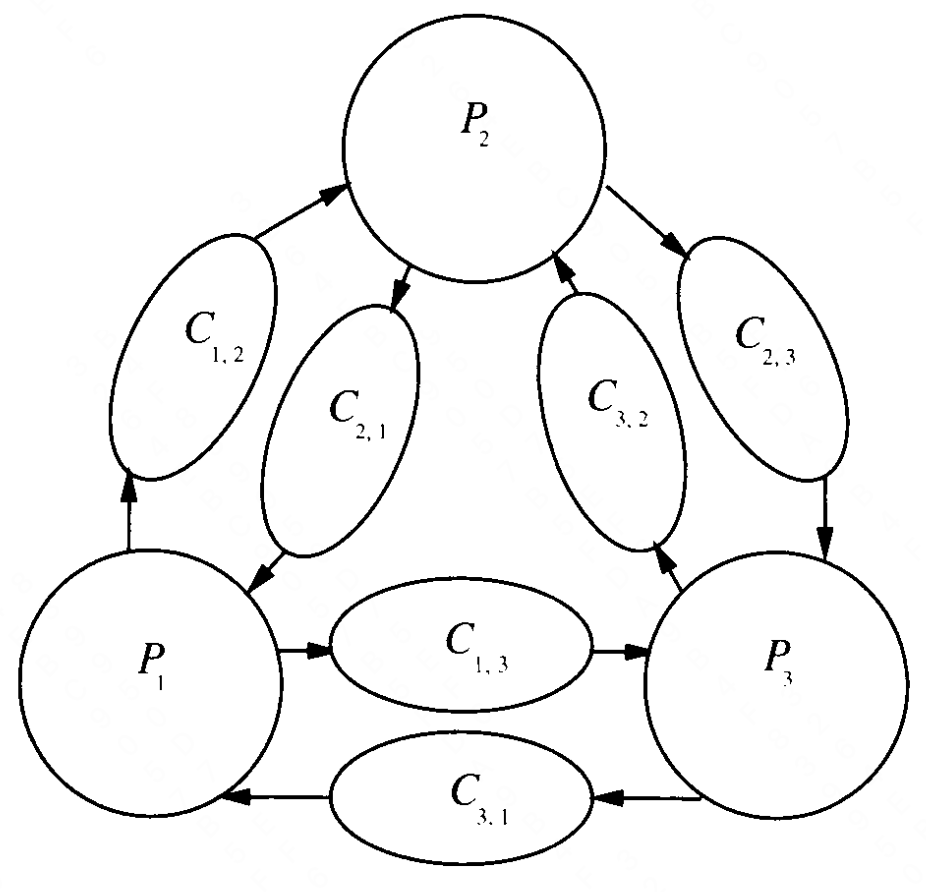
\includegraphics[width=.8\textwidth]{../images/DistributedAlgorithms/3.png}
\captionof{figure}{\label{8.3}Composition of \(P_i\)s and \(C_{i,j}\)s}
\end{center}

\begin{enumerate}
\item An \(init(v)_i\) input action, which deposits a value in \(P_i\)'s \(val(i)\) variable, \(val(i)_i\).
\item A \(send(v)_{i,j}\) output action, by which \(P_i\)'s value \(val(i)_i\) gets put into channel \(C_{i,j}\).
\item A \(receive(v)_{i,j}\) output action, by which the first message in \(C_{i,j}\) is removed and
simultaneously placed into \(P_j\)'s variable \(val(i)_j\).
\item A \(decide(v)_i\) output action, by which \(P_i\) announcs its current computed value.
\end{enumerate}
\end{examplle}

Given an execution \(\alpha=s_0,\pi_1,s_1,\dots\), of \(A\), let \(\alpha|A_i\) be the sequence
obtained by deleting each pair \(pi_r,s_r\) for which \(\pi_r\) is not an action of \(A_i\) and
replacing each remaining \(s_r\) by \((s_r)_i\).

\begin{theorem}[]
\label{8.1}
Let \(\{A_i\}_{i\in I}\) be a compatible collection of automata and let \(A=\prod_{i\in I}A_i\).
\begin{enumerate}
\item If \(\alpha\in execs(A)\), then \(\alpha|A_i\in execs(A_i)\) for every \(i\in I\).
\item If \(\beta\in traces(A)\), then \(\beta|A_i\in traces(A_i)\) for every \(i\in I\).
\end{enumerate}
\end{theorem}

\begin{proof}
\begin{enumerate}
\item Execution of any automaton \(A_j\) where \(j\neq i\) doesn't affect automaton \(A_i\).
\item Immediately
\end{enumerate}
\end{proof}

\begin{theorem}[]
\label{8.2}
Let \(\{A_i\}_{i\in I}\) be a compatible collection of automata and let \(A=\prod_{i\in I}A_i\).
Suppose \(\alpha_i\) is an execution of \(A_i\) for every \(i\in I\), and suppose \(\beta\) is a
sequence of actions in \(ext(A)\) s.t. \(\beta|A_i=traces(\alpha_i)\) for every \(i\in I\). Then there
is an execution \(\alpha\) of \(A\) s.t. \(\beta=trace(\alpha)\) and \(\alpha_i=\alpha|A_i\) for every
\(i\in I\).
\end{theorem}


\begin{theorem}[]
\label{8.3}
Let \(\{A_i\}_{i\in I}\)  be a compatible collection of automata and let \(A=\prod_{i\in I}A_i\).
Suppose \(\beta\) is a sequence of actions in \(ext(A)\). If \(\beta|A_i\in traces(A_i)\) for every
\(i\in I\), then \(\beta\in traces(A)\).
\end{theorem}
\subsubsection{Hiding}
\label{sec:orgc7bb28f}
If \(S\) is a signature and \(\Phi\subset out(S)\), then \(hide_\phi(S)\) is defined to be the new
signature \(S'\), where \(in(S')=in(S)\), \(out(S')=out(S)-\Phi\) and \(int(S')=int(S)\cup\Phi\).

If \(A\) is an automaton and \(\Phi\subseteq out(A)\), then \(hide_\Phi(A)\) is the automaton \(A'\)
obtained from \(A\) by replacing \(sig(A)\) with \(sig(A')=hide_\Phi(sig(A))\).
\subsubsection{Fairness}
\label{sec:orge95ebc8}
\index{fair}
An execution fragment \(\alpha\) of an I/O automaton \(A\) is said to be \textbf{fair} if the following
conditions hold for each class \(C\) of \(tasks(A)\):
\begin{enumerate}
\item If \(\alpha\) is finite, then \(C\) is not enabled in the final state of \(\alpha\)
\item If \(\alpha\) is infinite, then \(\alpha\) contains either infinitely many events from \(C\) or
infinitely many occurrences of states in which \(C\) is not enabled.
\end{enumerate}

We use the term \textbf{event} to denote the occurrence of an action in a sequence.

\begin{itemize}
\item We can understand the definition of fairness as saying that infinitely often, each task \(C\) is
given a turn. Whenever this happens, either an action of \(C\) gets performed or no action from
\(C\) could possibly be performed since no such action is enabled.
\item We can think of a finite fair execution as an execution at the end of which the automaton
repeatedly gives turns to all the tasks in round-robin order, but never succeeds in performing any
action since none are enabled in the final state. \label{P1}
\end{itemize}

We denote the set of fair executions of \(A\) by \(fairexecs(A)\). We say that \(\beta\) is a \textbf{fair
trace} of \(A\) if \(\beta\) is the trace of a fair execution of \(A\), and we denote the set of fair
traces of \(A\) by \(fairtraces(A)\).

\begin{examplle}[Fairness]
In Example \ref{8.1.3}, the first execution given is fair, because no \(receive\) action is enabled in
its final state. The second is not fair, because it is finite and a \(receive\) action is enabled in
the final state. The third is not fair, because it is infinite, contains no \(receive\) events, and
has \(receive\) actions enabled at every point after the first step.
\end{examplle}

\begin{theorem}[]
\label{8.4}
Let \(\{A_i\}_{i\in I}\) be a compatible collection of automata and let \(A=\prod_{i\in I}A_i\).
\begin{enumerate}
\item If \(\alpha\in fairexecs(A)\), then \(\alpha|A_i\in fairexecs(A_i)\) for every \(i\in I\).
\item If \(\beta\in fairtraces(A)\), then \(\beta|A_i\in fairtraces(A_i)\) for every \(i\in I\).
\end{enumerate}
\end{theorem}

\begin{proof}
\begin{enumerate}
\item If \(\alpha\in fairexecs(A)\).
\begin{itemize}
\item If \(\alpha\) is finite, then for each task \(C\), \(C\) is not enabled in the final state of
\(\alpha\), therefore each \(C|A_i\) is not enabled in the final state of \(\alpha|A_i\) too.
\item If \(\alpha\) is infinite, then blabla
\end{itemize}
Therefore \(\alpha|A_i\in fairexecs(A_i)\)
\item same
\end{enumerate}
\end{proof}

\begin{theorem}[]
\label{8.5}
Let \(\{A_i\}_{i\in I}\) be a compatible collection of automata and let \(A=\prod_{i\in I}A_i\).
Suppose \(\alpha_i\) is a fair execution of \(A_i\) for every \(i\in I\), and suppose \(\beta\) is a
sequence of actions in \(ext(A)\) s.t. \(\beta|A_i=trace(\alpha_i)\) for every \(i\in I\). Then there
is a fair execution \(\alpha\) of \(A\) s.t. \(\beta=trace(\alpha)\) and \(\alpha_i=\alpha|A_i\) for
every \(i\in I\).
\end{theorem}

\begin{theorem}[]
\label{8.6}
Let \(\{A_i\}_{i\in I}\) be a compatible collection of automata and let \(A=\prod_{i\in I}A_i\).
Suppose \(\beta\) is a sequence of actions in \(ext(A)\). If \(\beta|A_i\in fairexecs(A_i)\)  for
every \(i\in I\), then \(\beta\in fairexecs(A)\).
\end{theorem}

\begin{examplle}[Fairness]
Consider the fair executions of the system of three processes and three channels in Example \ref{8.2.1}.
In every fair execution, every message that is sent is eventually received.

In every fair execution containing least one \(init_i\) event for each \(i\), each process sends
infinitely many messages to each other processes and each process performs infinitely many \(decide\) steps

In every fair execution that does not contain at least one \(init\) event for each process, no process
ever performs a \(decide\) step.
\end{examplle}

\begin{theorem}[]
Let \(A\) be any I/O automaton.
\begin{enumerate}
\item If \(\alpha\) is a finite execution of \(A\), then there is a fair execution of \(A\) that starts
with \(\alpha\).
\item If \(\beta\) is a finite trace of \(A\), then there is a fair trace of \(A\) that starts with \(\beta\).
\item If \(\alpha\) is a finite execution of \(A\) and \(\beta\) is any sequence of input actions of
\(A\), then there is a fair execution \(\alpha\cdot\alpha'\) of \(A\) s.t. the sequence of input
actions in \(\alpha'\) is exactly \(\beta\)
\item If \(\beta\) is a finite trace of \(A\) and \(\beta'\) is any sequence of input actions of \(A\),
then there is a fair execution \(\alpha\cdot\alpha'\) of \(A\) s.t. \(trace(\alpha)=\beta\) and
s.t. the sequence of input actions in \(\alpha'\) is exactly \(\beta'\)
\end{enumerate}
\end{theorem}
\subsection{Inputs and Outputs for Problems}
\label{sec:org90a9043}
\subsection{Properties and Proof Methods}
\label{sec:org64c5bcc}
\subsubsection{Invariant Assertions}
\label{sec:orgefcc2d3}
\subsubsection{Trace Properties}
\label{sec:orge5fa665}
A \textbf{trace property} \(P\) consists of the following:
\begin{itemize}
\item \(sig(P)\), a signature containing no internal actions
\item \(traces(P)\), a set of (finite or infinite) sequences of actions in \(acts(sig(P))\)
\end{itemize}

That is, a trace property specifies both an external interface and a set (in other words, a property)
of sequences observed at that interface. We write \(acts(P)\) as shorthand for \(acts(sig(P))\), and
similarly \(in(P)\), and so on.

The statement that an I/O automaton \(A\) satisfies a trace property \(P\) can be mean either of two
different things:
\begin{enumerate}
\item \(extsig(A)=sig(P)\) and \(traces(A)\subseteq traces(P)\)
\item \(extsig(A)=sig(P)\) and \(fairtraces(A)\subseteq traces(P)\)
\end{enumerate}
The fact that \(A\) is input-enabled ensures that \(fairtraces(A)\) contains a response by \(A\) to
each possible sequence of input actions. If \(fairtraces(A)\subseteq traces(P)\), then all of the
resulting sequences must be included in the property \(P\).

\begin{examplle}[Automata and trace properties]
Consider automata and trace properties with input set \(\{0\}\) and output set \(\{1,2\}\). First
suppose that \(traces(P)\) is the set of sequences over \(\{0,1,2\}\) that include at least 1. Then
\(fairtraces(A)\subseteq traces(P)\) means that in every fair execution, \(A\) must output at least
one.

It is easy to design an I/O automaton for which this is the case - for example, it can include a task
whose entire job is to output 1. The fairness condition is used to ensure that this task actually does
get a change to output 1. On the other hand, there does not exist any automaton \(A\) for which
\(traces(A)\subseteq traces(P)\), because \(traces(A)\) always includes the empty string \(\lambda\),
which does not contain a 1.

Now suppose that \(traces(P)\) is the set of sequences over \(\{0,1,2\}\) that include at least one 0.
In this case, there is no I/O automaton \(A\) for which \(fairtraces(A)\subseteq traces(P)\), because
\(fairtraces(A)\) must contain some sequence that includes no inputs.
\end{examplle}

A countable collection \(\{P_i\}_{i\in I}\) of trace properties is \textbf{compatible} if their signatures are
compatible. Then the \textbf{composition} \(P=\prod_{i\in I}P_i\) is the trace property s.t.
\begin{itemize}
\item \(sig(P)=\prod_{i\in I}sig(P_i)\).
\item \(traces(P)\) is the set of sequences \(\beta\) of external actions of \(P\) s..t
\(\beta|acts(P_i)\in traces(P_i)\) for all \(i\in I\).
\end{itemize}
\subsubsection{Safety and Liveness Properties}
\label{sec:org12943e7}
\begin{definition}[]
A trace property \(P\) is a \textbf{trace safety property}, or a \textbf{safety property} for short, provided that \(P\)
satisfies the following conditions:
\begin{enumerate}
\item \(traces(P)\) is nonempty
\item \(traces(P)\) is \textbf{prefix-closed}, that is, if \(\beta\in traces(P)\) and \(\beta'\) is a finite
prefix of \(\beta\), then \(\beta'\in traces(P)\)
\item \(traces(P)\) is \textbf{limit-closed}, that is, if \(\beta_1,\beta_2,\dots\) is an infinite sequence of
finite sequences in \(traces(P)\), and for each \(i\), \(\beta_i\) is a prefix of \(\beta_{i+1}\),
then \(\beta=\bigcup_{i\in\omega}\beta_i\in traces(P)\).
\end{enumerate}
\end{definition}

\begin{examplle}[Trace safety property]
Suppose \(sig(P)\) consists of inputs \(init(v)\), \(v\in V\) and outputs \(decide(v)\), \(v\in V\).
Suppose \(traces(P)\) is the set of sequences of \(init\) and \(decide\) actions in which no
\(decide(v)\) occurs without a preceding \(init(v)\) (for the same \(v\)). Then \(P\) is a safety property.
\end{examplle}

\begin{proposition}[]
If \(P\) is a safe property, TFAE:
\begin{enumerate}
\item \(traces(A)\subseteq traces(P)\)
\item \(fairtraces(A)\subseteq traces(P)\)
\item finite traces of \(A\) are all in traces \(P\).
\end{enumerate}
\end{proposition}

\begin{proof}
\((2\Rightarrow(3)\): For any finite trace \(\beta\in traces(A)\), there is
\(\beta'\in fairtraces(A)\)  that starts in \(\beta\). Thus \(\beta\in traces(P)\) because of
prefix-closedness.

\((3)\Rightarrow(1)\): For any infinite trace \(\beta\in traces(A)\), we can have such a infinite
sequence of traces \(\beta_1,\beta_2,\dots\) of \(A\), where \(\beta_i\) is a prefix of
\(\beta_{i+1}\) for any \(i\), and \(\beta=\bigcup_{i\in\omega}\beta_i\). Therefore
\(\beta\in traces(P)\) because of limit-closedness.
\end{proof}

\begin{definition}[]
A trace property \(P\) is a \textbf{trace liveness property}, or a \textbf{liveness property} for short, provided that
every finite sequence over \(acts(P)\) has some extension in \(traces(P)\).
\end{definition}

\begin{examplle}[]
Suppose \(sig(P)\) consists of input \(init(v)\), \(v\in V\) and outputs \(decide(v)\), \(v\in V\).
Suppose \(traces(P)\) is the set of sequences \(\beta\) of \(init\) and \(decide\) actions in which,
for every \(init\) event in \(\beta\), there is some \(decide\) event occuring later in \(\beta\).
Then \(P\)  is a liveness property.
\end{examplle}

Often one wants to prove that \(fairtraces(A)\subseteq traces(P)\) for some automaton \(A\) and
liveness property \(P\). Methods based on \textbf{temporal logic} work well in practice for proving such
claims. Another method for proving liveness claims, which we call the \textbf{progress function method}, is
specially designed for proving that some particular goal is eventually reached.

\begin{theorem}[]
If \(P\) is both a safety property and a liveness property, then \(P\) is the set of all (finite and
infinite) sequence of actions in \(acts(P)\).
\end{theorem}

\begin{proof}
Suppose that \(P\) is both a safety and a liveness property and let \(\beta\) be an arbitrary sequence
of elements of \(acts(P)\). If \(\beta\) is finite, then since \(P\) is a liveness property, \(\beta\)
has some extension \(\beta'\) in \(traces(P)\). Then since \(P\) is a safety property, \(\beta\in
        traces(P)\).

If \(\beta\) is infinite, then for each \(i\ge 1\), define \(\beta_i\) to be the length \(i\) prefix
of \(\beta\). Then \(\beta\in traces(P)\).
\end{proof}

\begin{theorem}[]
If \(P\) is an arbitrary trace property with \(traces(P)\neq\emptyset\), then there exist a safety
property \(S\) and a liveness property \(L\) s.t.
\begin{enumerate}
\item \(sig(S)=sig(L)=sig(P)\).
\item \(traces(P)=traces(S)\cap traces(L)\)
\end{enumerate}
\end{theorem}

\begin{proof}
Let \(traces(S)\) be the prefix- and limit-closure of \(traces(P)\). Let
\begin{align*}
traces(L)=&traces(P)\\
&\cup\{\beta:\beta\text{ is a finite sequence and no extension of $\beta$ is in }traces(P)\}
\end{align*}
\begin{claim}
\(L\) is a liveness property
\end{claim}
Now \(traces(P)\subseteq traces(S)\cap traces(L)\). If there is \(\beta\in traces(S)\cap
        traces(L)\setminus traces(P)\),
then \(\beta\) is a finite sequence and no extension of \(\beta\) is in \(traces(P)\). \label{P2}
\end{proof}
\subsubsection{Compositional Reasoning}
\label{sec:orgb814512}
\begin{theorem}[]
\label{8.10}
Let \(\{A_i\}_{i\in I}\) be a compatible collection of automata and let \(A=\prod_{i\in I}A_i\). Let
\(\{P_i\}_{i\in I}\) be a (compatible) collection of trace properties and let \(P=\prod_{i\in I}P_i\)
\begin{enumerate}
\item If \(extsig(A_i)=sig(P_i)\) and \(traces(A_i)\subseteq traces(P_i)\) for every \(i\), then
\(extsig(A)=sig(P)\) and \(traces(A)\subseteq traces(P)\).
\item If \(extsig(A_i)=sig(P_i)\) and \(fairtraces(A_i)\subseteq traces(P_i)\) for every \(i\), then
\(extsig(A)=sig(P)\) and \(fairtraces(A)\subseteq traces(P)\).
\end{enumerate}
\end{theorem}

\begin{proof}
\begin{enumerate}
\item If \(\beta\in traces(A)\), then by Theorem \ref{8.1},
\(\beta|A_i\in traces(A_i)\subseteq traces(P_i)\) for every \(i\in I\). Then by Theorem \ref{8.3},
\(\beta\in traces(P)\).
\item 
\end{enumerate}
\end{proof}

\begin{examplle}[Satisfying a product trace property]
Consider the composed system of Example \ref{8.2.1}. Each process automaton \(P_i\) satisfies a trace
safety property that asserts that any \(decide_i\) event has a preceding \(init_i\) event. Also, each
channel automaton \(C_{i,j}\)  satisfies a trace safety property that asserts taht the sequence of
messages in \(receive_{i,j}\) events is a prefix of athe sequence of messages in \(send_{i,j}\)
events.

Then it follows from Theorem \ref{8.10} that the composed system satisfies the product trace safety
property. This means that in an trace of the combined system, the following hold:
\begin{enumerate}
\item For every \(i\), any \(decide_i\) event has a preceding \(init_i\) event
\item For every \(i\) and \(j\), \(i\neq j\), the sequence of messages in \(receive_{i,j}\) events is a
prefix of the sequence of messages in \(send_{i,j}\) events.
\end{enumerate}
\end{examplle}

Second, suppose that we want to show that a particular sequence of actions is a trace of a composed
system \(A=\prod_{i\in I}A_i\).  Theorem \ref{8.3} shows that it is enough to show taht the projection
of the sequence on each of the system components is a trace of that component. Theorem \ref{8.6} implies
an analogous result for fair traces.

Third, consider the compositional proof of safety properties. Suppose we want to show that a composed
system \(A=\prod_{i\in I}A_i\) satisfies a safety property \(P\). One strategy is to show that none of
the components \(A_i\) is the first to violate \(P\).

Let \(A\) be an I/O automaton and let \(P\) be a safety property with \(acts(P)\cap int(A)=\emptyset\)
and \(in(P)\cap out(A)=\emptyset\). We say that \(A\) \textbf{preserves} \(P\) if for every finite sequence
\(\beta\) of actions that does not include any internal actions of \(A\), and every \(\pi\in out(A)\),
the following holds: If \(\beta|acts(P)\in traces(P)\) and \(\beta\pi|A\in traces(A)\), then
\(\beta\pi|acts(P)\in traces(P)\). This says that \(A\) is not the first to violate \(P\), as long as
\(A\)'s environment only provides inputs to \(A\) in such a way that the cumulative behaviour
satisfies \(P\), then \(A\) will only perform outputs s.t. the cumulative behaviour satisfies \(P\).

The key fact about preservation of safety properties is that if all the components in a composed
system preserve a safety property, then so does the entire system. Moreover, if the composed system is
closed, then it actually satisfies the safety property.

\begin{theorem}[]
\label{8.11}
Let \(\{A_i\}_{i\in I}\) be a compatible collection of automata and let \(A=\prod_{i\in I}A_i\). Let
\(P\) be a safety property with \(acts(P)\cap int(A)=\emptyset\) and \(in(P)\cap out(A)=\emptyset\).
\begin{enumerate}
\item If \(A_i\) preserves \(P\) for every \(i\in I\), then \(A\) preserves \(P\)
\item If \(A\) is a closed automaton, \(A\) preserves \(P\), and \(acts(P)\subseteq ext(A)\), then
\(traces(A)|acts(P)\subseteq traces(P)\)
\item If \(A\) is a closed automaton, \(A\) preserves \(P\), and \(acts(P)=ext(A)\), then
\(traces(A)\subseteq traces(P)\).
\end{enumerate}
\end{theorem}
\subsubsection{Hierarchical Proofs}
\label{sec:org7a6bec5}
\subsection{Complexity Measures}
\label{sec:orge8e1b0f}
\section{Modelling \rom{3}: Asynchronous Shared Memory Model}
\label{sec:org3b99ff5}
\subsection{Shared Memory Systems}
\label{sec:org6b274e0}
We mode lthe entire system as one big I/O automaton \(A\).

As in the synchronous network model, we assume that the processes in the system are indexed by
\(1,\dots,n\). Suppose that each process \(i\) has an associated set of \textbf{states}, \(states_i\), among
which some are designated as \textbf{start states}, \(start_i\). Also suppose that each shared variable \(x\)
in the system has an associated set of \textbf{values}, \(values_x\), among which some are designated as the
\textbf{initial values}, \(initial_x\). Then each state in \(states(A)\) (the set of states of the system
automaton \(A\)) consists of a state in \(states_i\) for each process \(i\), plus a value in
\(values_x\) for each shared variable \(x\). Each state in \(start(A)\) consists of a state in
\(start_i\) for each process \(i\), plus a value in \(initial_x\) for each shared variable \(x\).

We assume that each action in \(acts(A)\) is associated with one of the processes. In addition, some
of the internal actions in \(int(A)\) may be associated with a shared variable. The input actions and
output actions associated with process \(i\) are used for interaction between process \(i\) and the
outside world; we say they occur on \textbf{port} \(i\). The internal actions of process \(i\) that do not have
an associated shared variable are used for local computation, while the internal actions of \(i\) that
are associated with shared variable \(x\) are used for performing operations on \(x\).

The set \(trans(A)\) of transitions has some locality restrictions, which model the process and shared
variable structure of the system.
\begin{enumerate}
\item Consider an action \(\pi\) that is associated with process \(i\) but with no variable; as we noted
above, \(\pi\) is used for local computation. Then only the state of \(i\) can be involved in any
\(\pi\) step. That is, the set of \(\pi\) transitions can be generated from some set of triples of
the form \((s,\pi,s')\), where \(s,s'\in states_i\), by attaching any combination of states for the
other processes and values for the shared variables to both \(s\) and \(s'\)
\item Consider an action \(\pi\) that is associated with both a process \(i\) and a variable \(x\);
\(\pi\) is used by \(i\) to perform an operation on \(x\). The set of \(\pi\) transitions can be
generated from some set of triples of the form \((s,v),\pi,(s',v')\), where \(s,s'\in states_i\)
and \(v,v'\in values_x\), by attaching any combination of states for the other processes and values
for the other shared variables. There is a \uline{technicality}: if \(\pi\) is associated with process
\(i\) and variable \(x\), then whether or not \(\pi\) is enabled should depend only on the state of
process \(i\)
\end{enumerate}

The task partitioon \(tasks(A)\) must be consistent with the process structure: that is, each
equivalence class (task) should include locally controlled actions of only one process.

\begin{examplle}[Shared memory system]
Let \(V\) be a fixed value set. Consider a shared memory system \(A\) consisting of \(n\) processes,
numbered \(1,\dots,n\), and a single shared variable \(x\) with values in \(V\cup\{unknown\}\),
initially \(unknown\). The inputs are of the form \(init(v)_i\), where \(v\in V\) and \(i\) is a
process index. The outputs are of the form \(decide(v)_i\), The internal actions are of the form
\(access_i\). All the actions with subscript \(i\) are associated with process \(i\), and in addition,
the \(access\) actions are associated with variable \(x\).

After process \(i\) receives an \(init(v)_i\) input, it accesses \(x\). If it finds \(x=unknown\),
then it writes its value \(v\) into \(x\) and decides \(v\). If it finds \(x=w\), where \(w\in V\),
then it does not write anything into \(x\), but decides \(w\).

Formally:

\textbf{States of \(i\)}:
\begin{align*}
&status\in\{idle,access,decide,done\}, \text{ initially } idle\\
&input\in V\cup\{unknown\},  \text{ initially } unknown\\
&output\in V\cup\{unknown\}, \text{ initially } unknown
\end{align*}
\textbf{Transitions of \(i\)}:
\begin{alignat*}{2}
&init(v)_i\hspace{3.5cm}&&decide(v)_i\\
&\quad\text{Effect:}&&\quad\text{Precondition:}\\
&\quad\quad input:=v&&\quad\quad status=decide\\
&\quad\quad\text{if }status=idle\text{ then}&&\quad\quad output=v\\
&\quad\quad\quad status:=access&&\quad\text{Effect:}\\
&&&\quad\quad status:=done\\
&access_i\\
&\quad\text{Precondition:}\\
&\quad\quad status=access\\
&\quad\text{Effect:}\\
&\quad\quad\text{if }x=unknown\text{ then }x:=input\\
&\quad\quad output:=x\\
&\quad\quad status:=decide
\end{alignat*}

There is one task per process, which contains all the \(access\) and \(decide\) actions for that
process.

It is not hard to see that in every fair execution \(\alpha\) of \(A\), any process that receives an
\(init\) input eventually performs a \(decide\) output. Moreover, every execution satisfies the
``agreement property'' that no two processes decide on different values, and the ``validity property''
that every decision value is the initial value of some process.
\end{examplle}
\section{Mutual Exclusion}
\label{sec:orgbe92367}
\subsection{Asynchronous Shared Memory Model}
\label{sec:orga8ef445}
The system is modelled as a collection of processes and shared variables,
with interactions. Each process \(i\) is a kind of state machine, with a set statesi of states and a subset \(start\) of \(states_i\) indicating the
start states, just as in the synchronous setting. However, now process \(i\) also has labelled
\(actions\), describing the activities in which it participates. These are classified as either
\(input\), \(output\), or \(internal\) actions. We further distinguish between two different kinds of
internal actions: those that involve the shared memory and those that involve strictly local
computation. If an action involves the shared memory, we assumethat it only involves one shared
variable.

There is a transition relation \(trans\) for the entire system, which is a set of \((s,\pi,s')\)
triples, where \(s\) and \(s'\) are \textbf{automaton states}, that is, combinations of states for all the
processes and values for all the shared variables, and where \(\pi\)  is the label of an input,
output, or internal action. We call these combinations of process states and variable values
``automaton states'' because  the entire system is modelled as a single automaton. The statement that
\((s,\pi,s')\in trans\) says that from automaton state \(s\) it is possible to go to automaton state
\(s'\) as a result of performing action \(\pi\).

We assume that input actions can always happen, that is, that the system is input-enabled. Formally,
this means that for every automaton state \(s\) and input action \(\pi\), there exists \(s'\) such
that \((s,\pi,s')\in trans\). In contrast, output and internal steps might be enabled only in a subset
of the states. The intuition behind the input-enabling property is that the input actions are
controlled by an arbitrary external user, while the internal and output actions are controlled by the
system itself.
\subsection{The Problem}
\label{sec:org13662b1}
The mutual exclusion problem involves the allocation of a single, indivisible, nonshareable resource
among \(n\) \textbf{users}, \(U_1,\dots,U_n\).

A user with access to the resource is modelled as being in a \textbf{critical region}, which is simply a
designated subset of its states. When a user is not involved in any way with the resource, it is said
to be in the \textbf{remainder region}. In order to gain admittance to its critical region, a user executes a
\textbf{trying protocol}, and after it is done with the resource, it executes an (often trivial) \textbf{exit protocol}.
This procedure can be repeated, so that each user follows a cycle, moving from its
\emph{remainder region} (R) to its \emph{trying region} (T), then to its \emph{critical region} (C), then to its \emph{exit
region} (E), and then back again to its remainder region.  

\begin{center}
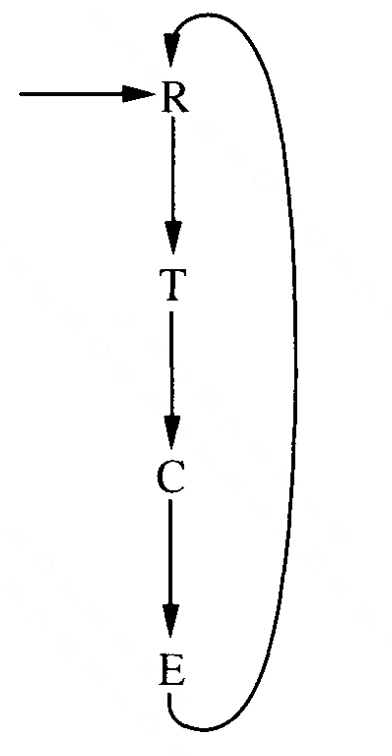
\includegraphics[width=.2\textwidth]{../images/DistributedAlgorithms/1.png}
\captionof{figure}{\label{10.2}The cycle of regions of a single user}
\end{center}

The inputs to process \(i\) are the \(try_i\) action, which models a request by user \(U_i\) for
access to the resource, and the \(exit_i\) action, which models an annoucement by user \(U_i\) that it
is done with the resource. The outputs of process \(i\) are \(crit_i\), which models the granting of
the resource to \(U_i\) and \(rem_i\), which tells \(U_i\) that it can continue with the reset of its
work. The \(try\), \(crit\), \(exit\), and \(rem\) actions are the only external actions of the shared
memory system. The processes are responsible for performing the trying and exit protocols. Each
process \(i\) acts as an ``agent'' on behalf of user \(U_i\).

Each of the users \(U_i\), \(1\le i\le n\), is modelled as a state machine (formally, an \textbf{I/O
automaton}) that communicates with its agent process using the \(try_i\), \(crit_i\), \(exit_i\) and
\(rem_i\) actions:
\begin{center}
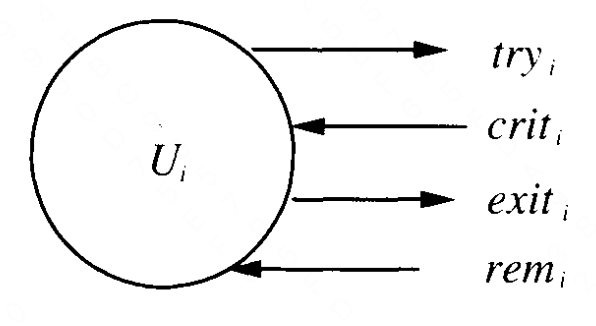
\includegraphics[width=.2\textwidth]{../images/DistributedAlgorithms/2.png}
\captionof{figure}{\label{10.3}External interface of user \(U_i\)}
\end{center}
The only thing that we assume about \(U_i\) is that it obeys the cyclic region protocol.
We define a sequence of \(try_i\), \(crit_i\), \(exit_i\) and \(rem_i\) actions to be \textbf{well-formed} for
user \(i\) if it is a prefix of the cyclically ordered sequence
\(try_i,crit_i,exit_i,rem_i,try_i,\dots\). Then we require that \(U_i\) \textbf{preserve} the \textbf{trace property}
defined by the set of sequences that are well-ordered for user \(i\).

In executions of \(U_i\) that do observe the cyclic order of actions, we say that \(U_i\) is
\begin{itemize}
\item in its \textbf{remainder region} initially and in between any \(rem_i\) event and the following \(try_i\) event
\item in its \textbf{trying region} in between \(try_i\) event and the following \(crit_i\) event
\item in its \textbf{critical region} in between any \(crit_i\) event and the following \(exit_i\) event. During
the time, \(U_i\) should be thought of as being free to use the resource
\item in its \textbf{exit region} in between any \(exit_i\) event and the following \(rem_i\) event
\end{itemize}


\begin{center}
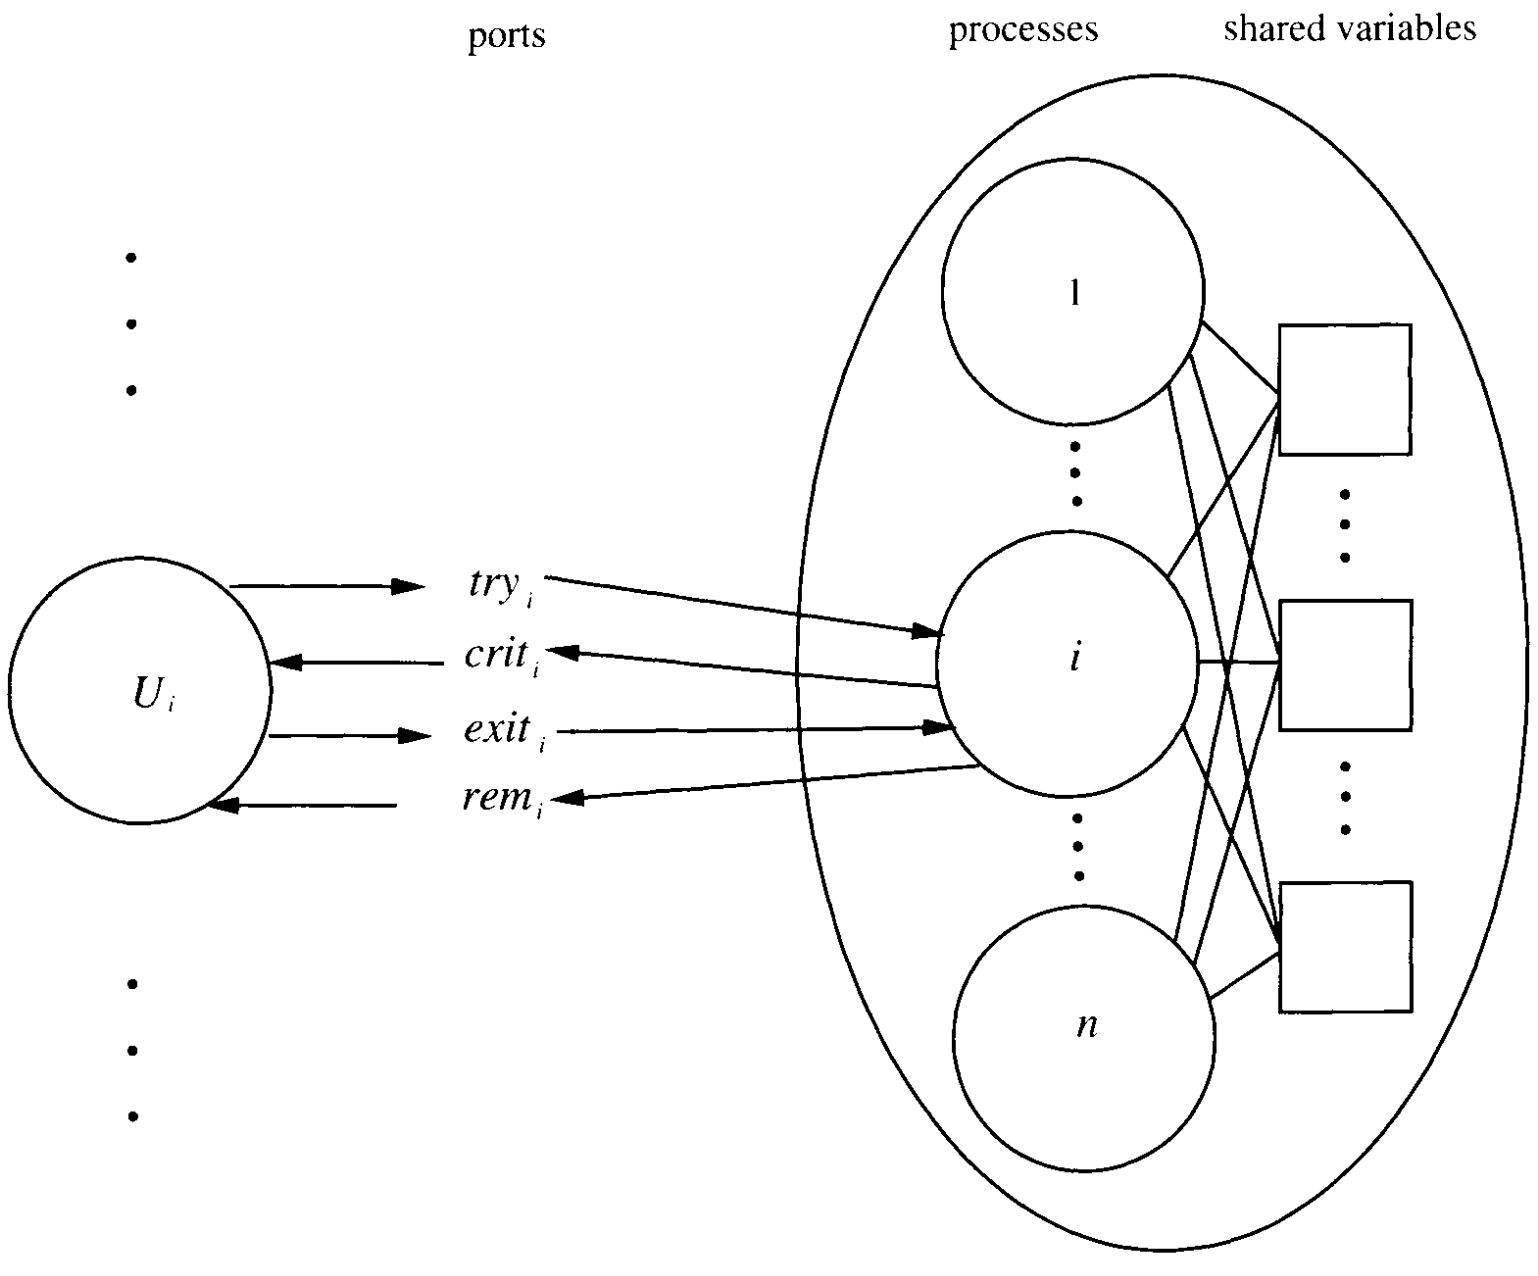
\includegraphics[width=.9\textwidth]{../images/DistributedAlgorithms/4.png}
\captionof{figure}{\label{10.4}Interactions between components for the mutual exclusion problem}
\end{center}

The combination of \(A\) and the users must satisfy the following conditions:
\begin{itemize}
\item \textbf{Well-formedness}: In any execution, and for any \(i\), the subsequence describing the interactions
between \(U_i\) and \(A\) is well-formed for \(i\).
\item \textbf{Mutual exclusion}: There is no reachable system state where more than one user is in the critical
region \(C\)
\item \textbf{Progress}: At any point in a \emph{fair execution}
\begin{enumerate}
\item (Progress for the trying region) If at least one user is in \(T\) and no user is in \(C\), then
at some later point some user enters \(C\)
\item (Progress for the exit region) If at least one user is in \(E\), then at some later point some
user enters \(R\).
\end{enumerate}
\end{itemize}

We say that a shared memory system \(A\) \textbf{solves the mutual exclusion problem} provided that it solves
it for every collection of users.


\begin{lemma}[]
\label{10.1}
Let \(A\) be an algorithm that solves the mutual exclusion problem. Let \(U_1,\dots,U_n\) be any
particular collection of users, and let \(B\) be the combination of \(A\) and the given collection of
users. Let \(s\) be a reachable state of \(B\).

If process \(i\) is in its trying or exit region in state \(s\), then some locally controlled action
of process \(i\) is enabled in \(s\).
\end{lemma}

\begin{proof}
WLOG, we may assume that each of the users always returns the resource.

Let \(\alpha\) be a finite execution of \(B\) ending in \(s\), and assume that process \(i\) is in
either its trying or exit region in state \(s\), and no locally controlled action of process \(i\) is
enabled in \(s\). Then we claim that no events involving \(i\) occur in any execution of \(B\) that
extends \(\alpha\), after the prefix \(\alpha\). This follows from the fact that enabling of locally
controlled actions is determined only by the local process state, plus the fact that well-formedness
prevents inputs to process \(i\) while process \(i\) is in \(T\) or \(E\).

Now let \(\alpha'\) be a fair execution of \(B\) that extends \(\alpha\), in which no \(try\) events
occur after the prefix \(\alpha\). Repeated use of the progress assumption, plus the fact that the
users always return the resource, imply that process \(i\) must eventually perform either a \(crit_i\)
or a \(rem_i\) action. But this contradicts the fact that \(\alpha'\) contains no further actions of \(i\).
\end{proof}
\subsection{Dijkstra's Mutual Exclusion Algorithm}
\label{sec:orgeea487d}
\subsubsection{The Algorithm}
\label{sec:orgc560804}
\begin{algorithm}[H]
\caption{DijkstraME algorithm}
\label{DijME}
\KwShared{\\\quad\(turn\in\{1,\dots,n\}\), initally arbitrary, writable and readable by all processes\\
        for every \(i\), \(1\le i\le n\):\\
        \quad\(flag(i)\in\{0,1,2\}\), initially 0, writable by process \(i\) and readable by all processes}\;
\KwProcess
\KwRem
\(try_i\)\;
\nlset{L}\label{zzzL}\(flag(i):=1\)\;
\While{\(turn\neq i\)}{
        \uIf{\(flag(turn)=0\)}{\(turn:=i\)\;}
}
\(flag(i):=2\)\;
\For{\(j\neq i\)}{
        \uIf{\(flag(j)=2\)}{\KwGoTo \ref{zzzL}\;}
}
\(crit_i\)\;
\KwCrit
\(exit_i\)\;
\(flag(i):=0\)\;
\(rem_i\)\;
\end{algorithm}

The \(turn\) variable is a \(multi\text{-}writer\)/\(multi\text{-}reader\) register. Each \(flag(i)\) is a
\(single\text{-}writer\)/\(multi\text{-}reader\) register.


The state of each process should consist of the values of its local variables plus some other
information that is not represented explicitly in the code, including
\begin{itemize}
\item temporary variables needed to remember values just read from shared variables
\item a program counter
\item temporary variables introduced by the flow of control of the program
\item a region designation, \(R\), \(T\), \(C\), or \(E\)
\end{itemize}


The unique start state of each process should consist of specified initial values for local variables,
arbitrary values for temporary variables, and the program counter and the region designation
indicating the remainder region.

There are some ambiguities in the code that need to be resolved in the automaton.
\begin{enumerate}
\item Although the code describes the changes to the local and shared variables, it does not say
explicitly what happens to the implicit variables
\item The code also does not specify exactly which portions of the code comprise indivisible steps.
\end{enumerate}


\begin{Block}{\textit{DijkstraME} algorithm (rewritten)}
\textbf{Shared variables}:\\
\(turn\in\{1,\dots,n\}\), initially arbitrary\\
for every \(i\), \(1\le i\le n\):\\
\indent\(flag(i)\in\{0,1,2\}\), initially 0

\noindent \textbf{Actions of \(i\)}:\\
\begin{tabular}{ll}
Input:\hspace{3cm} & Internal:\\
\(\qw try_i\) & \(\qw set\text{-}flag\text{-}1_i\)\\
\(\qw exit_i\) & \(\qw test\mhyphen turn_i\)\\
Output: & \(\qw test\mhyphen flag(j)_i,1\le j\le n,j\neq i\)\\
\(\qw crit_i\) & \(\qw set\mhyphen turn_i\)\\
\(\qw rem_i\) & \(\qw set\mhyphen flag\mhyphen 2_i\)\\
 & \(\qw check(j)_i,1\le j\le n,j\neq i\)\\
 & \(\qw reset_i\)\\
\end{tabular}


\noindent \textbf{States of \(i\)}:\\
\(pc\in\{\rem,\setflagi,\testturn,\testflag(j),\setturn,\allowbreak \setflagii,check,\\\leavetry,crit,reset,\leaveexit\}\),
initially \(rem\).

\(S\), a set of process indices, initially \(\emptyset\).

\noindent \textbf{Transitions of \(i\)}:

\resizebox{0.9\linewidth}{!}{
        \begin{tabular}{l|l}
\(try_i\) & \(\setturn_i\)\\
\qw Effect: & \qw Precondition:\\
\(\qw\qw pc:=\setflagi\) & \(\qw\qw pc=\setturn\)\\
 & \qw Effect:\\
\(\setflagi_1\) & \(\qw\qw turn:=i\)\\
\qw Precondition: & \(\qw\qw pc:=\setflagii\)\\
\(\qw\qw pc=\setflagi\) & \\
\qw Effect: & \(\setflagii_i\)\\
\(\qw\qw flag(i):=1\) & \qw Precondition:\\
\(\qw\qw pc:=\testturn\) & \(\qw\qw pc=\setflagii\)\\
 & \qw Effect:\\
\(\testturn_i\) & \(\qw\qw flag(i):=2\)\\
\qw Precondition: & \(\qw\qw S:=\{i\}\)\\
\(\qw\qw pc=\testturn\) & \(\qw\qw pc:=check\)\\
\qw Effect: & \\
\qw\qw if \(turn=i\) then \(pc:=\setflagii\) & \(check(j)_i\)\\
\qw\qw else \(pc:=\testflag(turn)\) & \qw Precondition:\\
 & \(\qw\qw pc=check\)\\
\(\testflag(j)_i\) & \(\qw\qw j\notin S\)\\
\qw Precondition: & \qw Effect:\\
\(\qw\qw pc=\testflag(j)\) & \qw\qw if \(flag(j)=2\) then\\
\qw Effect: & \(\qw\qw\qw S:=\emptyset\)\\
\qw\qw if \(flag(j)=0\) then \(pc:=\setturn\) & \(\qw\qw\qw pc:=\setflagi\)\\
\qw\qw else \(pc:=\testturn\) & \qw\qw else\\
 & \(\qw\qw\qw S:=S\cup\{j\}\)\\
\(crit_i\) & \qw\qw\qw\qw if \(\abs{S}=n\) then \(pc:=\leavetry\)\\
\qw Precondition: & \\
\(\qw\qw pc=\leavetry\) & \(reset_i\)\\
\qw Effect: & \qw Precondition:\\
\(\qw\qw pc:=crit\) & \qw\qw\(pc=reset\)\\
 & \qw Effect:\\
\(exit_i\) & \qw\qw \(flag(i):=0\)\\
\qw Effect: & \qw\qw \(S:=\emptyset\)\\
\qw\qw\(pc:=reset\) & \qw\qw \(pc:=\leaveexit\)\\
 & \\
 & \(rem_i\)\\
 & \qw Precondition:\\
 & \qw\qw \(pc=\leaveexit\)\\
 & \qw Effect:\\
 & \qw\qw \(pc:=rem\)\\
        \end{tabular}
}
\end{Block}
\subsubsection{A Correctness Argument}
\label{sec:org044f409}
\begin{lemma}[]
DijkstraME guarantees well-formedness for each user.
\end{lemma}

\begin{proof}
By inspection of the code, it is easy to check that DijkstraME preserves well-formedness for each
user. Since, by assumption, the users also preserve well-formedness, Theorem \ref{8.11} implies that the
system produces only well-formed sequences.
\end{proof}

\begin{lemma}[]
\label{10.3}
DijkstraME satisfies mutual exclusion
\end{lemma}

\begin{proof}
By contradiction. Assume that \(U_i\) and \(U_j\), \(i\neq j\), are simultaneouly in region \(C\) in
some reachable state. Consider the execution that leads to this state. By the code, both \(i\) and
\(j\) perfrom \(\setflagii\) steps before entering their critical area. Consider the last such step
for each process and assume, without loss of generality, that \(\setflagii_i\) comes first. Then
\(flag(i)\) is 2 from that point until \(i\) leaves \(C\), contradicting the fact that \(j\) enters \(C\).

\begin{center}
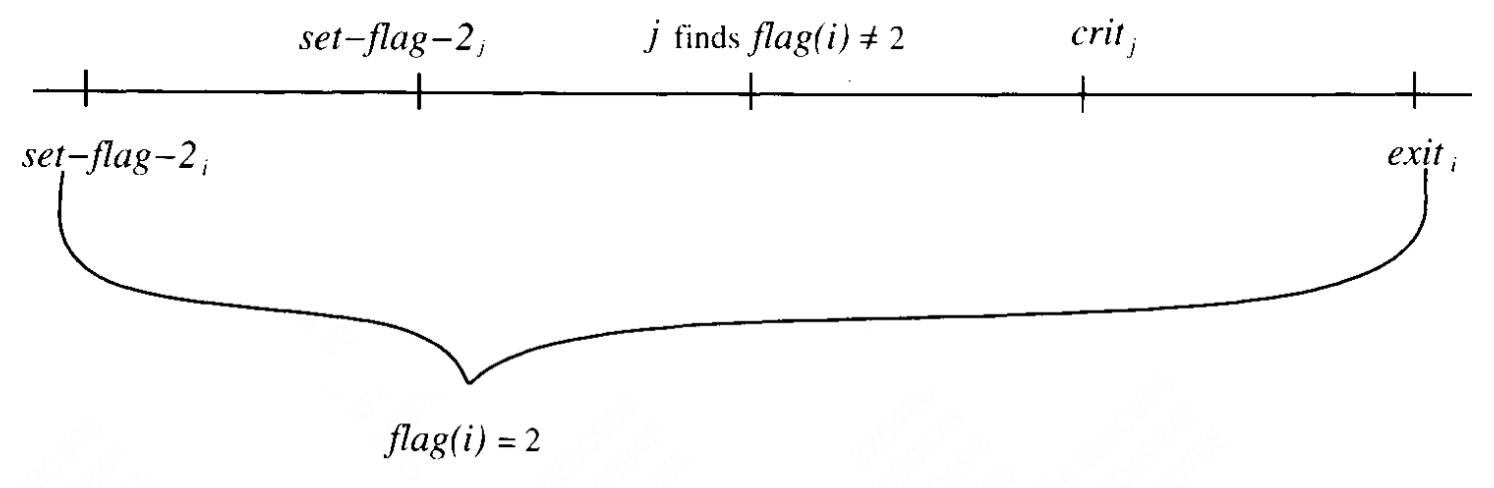
\includegraphics[width=.8\textwidth]{../images/DistributedAlgorithms/6.png}
\captionof{figure}{\label{105}Order of events in the proof of Lemma \ref{10.3}}
\end{center}
\end{proof}

\begin{lemma}[]
DijkstraME guarantees progress.
\end{lemma}

\begin{proof}
Progress of exit region is easy.

We consider the progress condition for the trying region. Suppose for the sake of contradiction that \(\alpha\)
is a fair execution that reaches a point where there is at least one user in \(T\) and no user in \(C\), and
suppose that after this point, no user ever enters \(C\).

Any process in \(E\) keeps taking steps, so after at most two steps, it must reach \(R\). So after
some point in \(\alpha\), every process must be in \(T\) or \(R\). Second, since there are only
finitely many processes in the system, after some point in \(\alpha\), no new processes enter \(T\).
Thus, after some point in \(\alpha\), every process is in \(T\) or \(R\), and no process every again
changes region. This implies that \(\alpha\) has a suffix \(\alpha_1\) in which there is a fixed
nonempty set of processes in \(T\), continuing to take steps forever, and no region changes occur.
Call these processes \textbf{contenders}.

Note that after at most a single step in \(\alpha_1\), each contender \(i\) ensures that
\(flag(i)\ge1\)  and it remains \(\ge 1\) for the rest of \(\alpha_1\). So we can assume, WLOG, that
\(flag(i)\ge 1\) for all contenders throughout \(\alpha_1\).

\begin{claim}
In \(\alpha_1\), turn eventually acquires a contender's index.
\end{claim}

\#+BEGIN\textsubscript{proof}
Suppose not, that is, suppose the value of \(turn\) remains equal to the index of a non-contender
throughout \(\alpha_1\). Consider any contender \(i\).

If \(pc_i\) reaches \(\testturn\), which is happened since \(i\) fails to enter \(C\), then
\(\testturn_i\) finds that \(turn\) equal to some \(j\neq i\).
Then it performs a \(\testturn_i\) and finds \(flag(j)=0\). Process \(i\) therefore performs
\(\setturn_i\), setting \(turn\) to \(i\).
\end{proof}
Once \(turn\) is set to a contender's index, it is always thereafter equal to \emph{some} contender's index.
Then any later \(\testturn\) and subsequent \(\testflag\) yield \(flag(turn)\ge 1\). Thus, \(turn\)
will not changed as a result of these tests. Therefore, eventually \(turn\) stabilizes to a final
indx. Let \(\alpha_2\) be a suffix of \(\alpha_1\) in which the value of \(turn\) is stablized at some
contender's index, say \(i\).

Next, we claim that in \(\alpha_2\), any contender \(j\neq i\) eventually ends up with its program
counter looping forever between \(\testturn\) and \(\testflag\). So let \(\alpha_3\) be a suffix of
\(\alpha_2\) where all contenders other than \(i\)  loop forever between \(\testturn\) and
\(\testflag\). Note that this means that all contenders other than \(i\) have their flag variables equal
to 1 throughout \(\alpha_3\).

We conclude the argument by claiming that in \(\alpha_3\), process \(i\) (the one whose index is in
turn) has nothing to stand in the way of its reaching \(C\).
\#+END\textsubscript{proof}

\begin{theorem}[]
DijkstraME solves the mutual exclusion problem.
\end{theorem}
\subsubsection{An Assertion Proof of the Mutual Exclusion Condition}
\label{sec:org8cf58d3}
\begin{proof}[another proof of Lemma \ref{10.3}]
\begin{assertion}
\label{10.3.1}
In any reachable system state, \(\abs{\{i:pc_i=crit\}}\le 1\)
\end{assertion}

\begin{assertion}
\label{10.3.2}
In any reachable system state, if \(pc_i\in\{\leavetry,crit,reset\}\), then \(\abs{S_i}=n\)
\end{assertion}

\begin{assertion}
\label{10.3.3}
In any reachable system state, there do not exist \(i\) and \(j\), \(i\neq j\), s.t. \(i\in S_j\) and
\(j\in S_i\).
\end{assertion}

If both Assertions \ref{10.3.2} and \ref{10.3.3} are true, then Assertion \ref{10.3.1} follows.

Assertion \ref{10.3.2} is easy.

\begin{assertion}
\label{10.3.4}
In any reachable system state, if \(S_i\neq\emptyset\), then \(pc_i\in\{check,\leavetry,crit,reset\}\).
\end{assertion}

\begin{assertion}
\label{10.3.5}
In any reachable system state, if \(pc_i\in\{check,\leavetry,crit,reset\}\), then \(flag(i)=2\)
\end{assertion}

Putting these together, we see that:
\begin{assertion}
\label{10.3.6}
In any reachable system state, if \(S_i\neq\emptyset\), then \(flag(i)=2\).
\end{assertion}

Now we can prove Assertion \ref{10.3.3}, again by induction on the length of an execution. For the
inductive step, the only event that could cause a violation is one that adds an element \(j\) to
\(S_i\) for some \(i\) and \(j\), \(i\neq j\), that is, a \(check(j)_i\). Then it must be that
\(flag(j)\neq 2\) when this event occurs. But then \(S_j=\emptyset\), so \(i\notin S_j\).
\end{proof}
\subsubsection{Running Time}
\label{sec:orgadb5429}
We impose:
\begin{itemize}
\item an upper bound of \(l\) on the time between successive steps of each process (when these steps are
enabled);
\item all the precondition-effect code for one action is assumed to comprise a single step.
\item an upper bound of \(c\) on the maximum time that any user spends in the critical region.
\end{itemize}

In terms of these assumed bounds, we can deduce upper bounds for the time required for interesting
activity to occur. 

\begin{theorem}[]
\label{10.7}
In DijkstraME, suppose that at a particular time some user is in \(T\) and no user is in \(C\). Then
within \(O(ln)\), some user enters \(C\)
\end{theorem}

\begin{proof}
Suppose the lemma is false and consider an execution in which, at some point, process \(i\) is in
\(T\) and no process is in \(C\), and in which no process enters \(C\) for time at  least \(kln\), for
some particular large constant \(k\).

First, it is easy to see that the time elapsed from the starting point of the analysis until there is
no process either in \(C\) or \(E\) is at most \(O(l)\).

Second, we claim that the additional time until process \(i\) performs a \(\testturn_i\) is at most
\(O(ln)\).  This is because \(i\) can at worst spend this much time checking flags in the second stage
before returning to \(\setflagi\).

Third, we claim that the additional time from when process i does \(\testturn_i\) until the value of
turn is a contender index is at most \(O(l)\).

Fourth, after an additional time \(O(l)\), a point is reached at which the value of \(turn\) has
stablized to the index of some particular contender, say \(j\).

Fifth, we claim that by an additional time \(O(ln)\), all contenders other than \(j\) will have their
program counters in \(\testturn, \testflag\).

Sixth and finally, within an additional time \(O(ln)\), \(j\) must succeed in entering \(C\)

\begin{center}
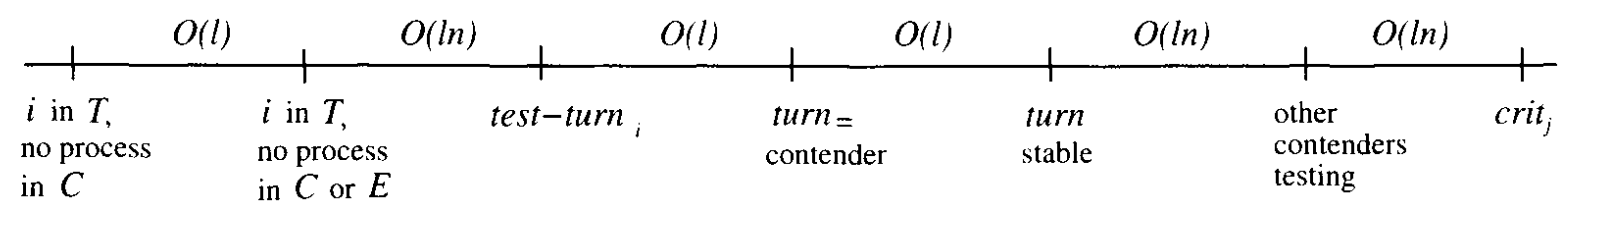
\includegraphics[width=.99\textwidth]{../images/DistributedAlgorithms/7.png}
\captionof{figure}{\label{}Order of events and time bounds in proof of Theorem \ref{10.7}}
\end{center}
\end{proof}
\subsection{Stronger Conditions for Mutual Exclusion Algorithms}
\label{sec:org643b83c}
In order to distinguish these two types of fairness, we will call the fair execution of process steps
and user automata steps \textbf{low-level fairness}, and the fair granting of the resource \textbf{high-level fairness}.

Another not-so-attractive property of Dijkstra's algorithm is that it uses a shared
\emph{multi-writer/multi-reader} register (turn). Such a variable is difficult and expensive to implement in
many kinds of multiprocessor systems (as well as in nearly all message-passing systems). It would be
better to design algorithms that use only \emph{single-writer/multi-reader} registers, or even better,
\emph{single-writer/single-reader} registers.

Each of these properties is stated for a particular mutual exclusion algorithm \(A\) composed with a
particular collection \(U_1,\dots,U_n\) of users.

\textbf{Lockout-freedom}: In any low-level-fair execution, the following hold:
\begin{enumerate}
\item (Lockout-freedom for the trying region) If all users always return the resource, then any user that
reaches \(T\) eventually enters \(C\).
\item (Lockout-freedom for the exit region) Any user that reaches \(E\) eventually enters \(R\).
\end{enumerate}

\textbf{Time bound \(b\)}: In any low-level-fair execution with associated times, the following hold:
\begin{enumerate}
\item (Time bound \(b\) for the trying region) If each user always returns the resource within time \(c\)
of when it is granted, and the time between successive steps of each process in \(T\) or \(E\) is
at most \(l\), then any user that reaches \(T\) enters \(C\) within time \(b\).
\item (Time bound \(b\) for the exit region) If the time between successive steps of each process in
\(T\) or \(E\) is at most \(g\), then any user that reaches \(E\) enters \(R\) within time \(b\).
\end{enumerate}

\textbf{Number of bypasses \(a\)}: Consider any interval of an execution starting when a process \(i\) has
performed a locally controlled step in \(T\), and throughout which it remains in \(T\). During this
interval, any other user \(j\), \(j\neq i\), can only enter \(C\) at most \(a\) times.

\begin{theorem}[]
Let \(A\) be a mutual exclusion algorithm, let \(U_1,\dots,U_n\) be a collecion of users, and let
\(B\) be the composition of \(A\) with \(U_1,\dots,U_n\). If \(B\) has any finite bypass round and is
lockout-free for the exit region, then \(B\) is lockout-free.
\end{theorem}

\begin{proof}
Consider a low-level-fair execution of \(B\) in which all users always return the resource, and
suppose that at some point in the execution, \(i\) is in \(T\). Assume for the sake of contradiction
that \(i\) never enters \(C\). Lemma \ref{10.1} implies that eventually \(i\) must perform a locally
controlled action in that trying region, if it has not already done so. Repeated use of the progress
condition and of the assumption that users always return the resource together imply that infinitely
many total region changes occur. But then some process other than \(i\) enters \(C\) an infinite
number of times while \(i\) remains in \(T\), which violates the bypass bound.
\end{proof}

\begin{theorem}[]
Let \(A\) be a mutual exclusion algorithm, let \(U_1,\dots,U_n\) be a collection of users, and let
\(B\) be the composition of \(A\) with \(U_1,\dots,U_n\). If \(B\) has any time bound \(b\), then
\(B\) is lockout-free.
\end{theorem}
\subsection{Lockout-Free Mutual Exclusion Algorithms}
\label{sec:orgbd48a96}
\subsubsection{A Two-Process Algorithm.}
\label{sec:orgd6a72ea}
If \(i\in\{0,1\}\), we write \(\bari\) to indicate \(1-i\).

\begin{Block}{\textit{Peterson2P} algorithm}
\textbf{Shared variables}:\\
\(turn\in\{0,1\}\), initially arbitrary, writable and readable by all processes

For every \(i\in\{0,1\}\):
\qw\(flag(i)\in\{0,1\}\), initially 0, writable by \(i\) and readable by \(\bari\)

\textbf{Process \(i\)}:\\
\begin{algorithm}[H]
\caption{}
\KwRem
\(try_i\)\;
\(flag(i):=1\)\;
\(turn:=i\)\;
wait for \(flag(\bari)=0\) or \(turn\neq i\)\;
\(crit_i\)
\KwCrit
\(exit_i\)\;
\(flag(i):=0\)\;
\(rem_i\)\;
\end{algorithm}
\end{Block}

\begin{Block}{\textit{Peterson2P} algorithm (rewritten)}
\textbf{Shared variables}:\\
\(turn\in\{0,1\}\), initially arbitrary

\noindent for every \(i\in\{0,1\}\):\\
\indent\(flag(i)\in\{0,1\}\), initially 0

\noindent \textbf{Actions of \(i\)}:\\
\begin{tabular}{l|l}
Input:&Internal:\\
\qw\(try_i\)&\qw\(\setflag_i\)\\
\qw\(exit_i\)&\qw\(\setturn_i\)\\
Output:&\qw\(\checkflag_i\)\\
\qw\(crit_i\)&\qw\(\checkturn_i\)\\
\qw\(rem_i\)&\qw\(reset_i\)
\end{tabular}

\noindent \textbf{States of \(i\)}:\\
\(pc\in\{rem,\setflag,\setturn,\checkflag,\checkturn,\leavetry,crit,reset,\\\leaveexit\}\), initially
\(rem\)

\noindent \textbf{Transitions of \(i\)}:\\

\begin{center}\begin{tikzpicture}[scale=0.6,transform shape,
every node/.style={rectangle,draw,rounded corners,drop shadow,fill=blue!5},
arr/.style = {-{Stealth[length=1mm, width=1mm]},shorten >=1pt,rounded corners=10pt},]
\node (try)
{$\begin{aligned}
&try_i\\
&\qw\text{Effect:}\\
&\qw\qw pc:=\setflag
\end{aligned}$};
\node (setflag) [below=of try]
{$\begin{aligned}
&\setflag_i\\
&\qw\text{Precondition}:\\
&\qw\qw pc=\setflag\\
&\qw\text{Effect}:\\
&\qw\qw flag(i):=1\\
&\qw\qw pc:=\setturn
 \end{aligned}$};
\node (setturn) [below=of setflag]
{$\begin{aligned}
&\setturn_i\\
&\qw\text{Precondition:}\\
&\qw\qw pc=\setturn\\
&\qw\text{Effect:}\\
&\qw\qw turn:=i\\
&\qw\qw pc:=\checkflag
 \end{aligned}$};
\node (checkflag) [below=of setturn]
{$\begin{aligned}
&\checkflag_i\\
&\qw\text{Precondition:}\\
&\qw\qw pc=\checkflag\\
&\qw\text{Effect:}\\
&\qw\qw \text{ if }flag(\bari)=0\text{ then}\\
&\qw\qw\qw pc:=\leavetry\\
&\qw\qw\text{else}\\
&\qw\qw\qw pc:=\checkturn
 \end{aligned}$};
\node (crit) [below=of checkflag]
{$\begin{aligned}
&crit_i\\
&\qw\text{Precondition:}\\
&\qw\qw pc=\leavetry\\
&\qw\text{Effect:}\\
&\qw\qw pc:=crit
 \end{aligned}$};
\node[right=of checkflag] (checkturn)
{$\begin{aligned}
&\checkturn_i\\
&\qw\text{Precondition:}\\
&\qw\qw pc=\checkturn\\
&\qw\text{Effect:}\\
&\qw\qw\text{ if }turn\neq i\text{ then}\\
&\qw\qw\qw pc:=\leavetry\\
&\qw\qw\text{else}\\
&\qw\qw\qw pc:=\checkflag
 \end{aligned}$};
\node[right =5cm of try] (exit)
{$\begin{aligned}
&exit_i\\
&\qw\text{Effect:}\\
&\qw\qw pc:=reset\\
 \end{aligned}$};
\node[below=of exit] (reset)
{$\begin{aligned}
&reset_i\\
&\Precondition\\
&\qw\qw pc=reset\\
&\Effect\\
&\qw\qw flag(i):=0\\
&\qw\qw pc:=\leaveexit
 \end{aligned}$};
\node[below=of reset] (rem)
{$\begin{aligned}
&rem_i\\
&\Precondition\\
&\qw\qw pc=\leaveexit\\
&\Effect\\
&\qw\qw pc:=rem
 \end{aligned}$};
\path[->,arr] (try) edge (setflag)
                         (setflag) edge (setturn)
                         (setturn) edge (checkflag)
                         (checkflag) edge (crit)
                        (checkflag)  edge (checkturn)
                         (exit) edge (reset)
                         (reset) edge (rem)
                        (checkturn) edge (checkflag)
                        (checkturn.south) edge (crit.east);
\end{tikzpicture}\end{center}
\end{Block}

\begin{lemma}[]
Peterson2P satisfies mutual exclusion
\end{lemma}

\begin{proof}
\begin{assertion}
In any reachable system state, if \(flag(i)=0\), then \(pc_i\in\{\leaveexit,rem,\setflag\}\)
\end{assertion}

\begin{assertion}
\label{10.5.2}
In any reachable system state, if \(pc_i\in\{\leavetry,crit,reset\}\), and
\(pc_{\bari}\in\{\checkflag,\checkturn,\leavetry,crit,reset\}\), then \(turn\neq i\).
\end{assertion}
That is, if \(i\) has won the competition, and if \(\bari\) is a competitor, then the \(turn\)
variable is set favorably for \(i\).

Suppose both \(i\) and \(\bari\) are in \(C\), then Assertion \ref{10.5.2}, applied twice for \(i\) and
\(\bari\), implies that both \(turn\neq i\) and \(turn\neq\bari\).
\end{proof}

\begin{lemma}[]
Peterson2P guarantees progress.
\end{lemma}

\begin{proof}
Suppose \(\alpha\) is a low-level-fair execution that reaches a point where at least one of the
processes, say \(i\), is in \(T\) and neither process is in \(C\), and suppose that after this point,
neither process ever enters \(C\).
\begin{enumerate}
\item If \(\bari\) is in \(T\) sometime after the given point in \(\alpha\), then both processes must get
stuck in their \(check\) loops, which is impossible
\item If \(\bari\) is never in \(T\) after the given point in \(\alpha\), we can show that
\(flag(\bari)\) eventually becomes and stays equal to 0.
\end{enumerate}
\end{proof}

\begin{lemma}[]
Peterson2P is lockout-free
\end{lemma}

\begin{proof}
Consider the lockout-freedom for trying region.

Suppose the contrary, that is, that at some point in execution \(\alpha\), process \(i\) is in \(T\)
after having performed \(\setflag_i\), and thereafter, while \(i\) remains in \(T\), process \(\bari\)
enters \(C\) three times.

Note that in each of the second and third times, it must be that \(\bari\) first sets \(turn:=\bari\)
and then sees \(turn=i\); it cannot see \(flag(i)=0\). This means that there are at least two
occurrences of \(\setturn_i\) after the given point in \(\alpha\). But \(\setturn_i\) is only
performed once.
\end{proof}

Let \(l\) and \(c\) be upper bounds on process step time and critical section time, respectively.

\begin{theorem}[]
In Peterson2P, the time from when a particular process \(i\) enters \(T\) until it enters \(C\) is
most \(c+O(l)\).
\end{theorem}
\subsubsection{An \texorpdfstring{\(n\)}{n}-Process Algorithm}
\label{sec:orgc2e37b1}
For \(n\) processes, we can use the idea of the \emph{Peterson2P} algorithm iteratively, in a series of
\(n-1\) competitions at levels \(1,2,\dots,n-1\). At each successive competition, the algorithm
ensures that there is at least one \textbf{loser}. Thus, all \(n\) processes may compete in the level 1
competition, but at most \(n-1\) processes can win.

\begin{Block}{}
\noindent \textbf{Shared variables}:\\
\noindent for every \(k\in\{1,\dots,n-1\}\):
\indent\(turn(k)\in\{1,\dots,k\}\), initially arbitrary
\noindent for every \(i\), \(1\le i\le n\):
\indent\(flag(i)\in\{0,\dots,n-1\}\), initially 0

\noindent \textbf{Process \(i\)}:\\
\begin{algorithm}[H]
\caption{}
\KwRem
\(try_i\)\;
\For{\(k\in\{1,\dots,n-1\}\)}{
        \(flag(i):=k\)\;
        \(turn(k):=i\)\\
        wait for \([\forall j\neq i:flag(j)<k]\) or \([turn(k)\neq i]\)\;
}
\KwCrit
\(exit_i\)\;
\(flag(i):=0\)\;
\(rem_i\)\;
\end{algorithm}
\end{Block}

Ambiguities:
\begin{itemize}
\item one of the conditions in the waitfor statement involves the flag variables for all the other processes.
\item we need to specify some conditions on the order in which process i checks the various \(flag\) variables and the \(turn(k)\) variable,
\end{itemize}

\begin{Block}{}
\noindent \textbf{Shared variables}:\\
\noindent for every \(k\in\{1,\dots,n-1\}\):
\indent\(turn(k)\in\{1,\dots,k\}\), initially arbitrary
\noindent for every \(i\), \(1\le i\le n\):
\indent\(flag(i)\in\{0,\dots,n-1\}\), initially 0

\noindent \textbf{Actions of \(i\)}:\\
\begin{tabular}{ll}
Input:&Internal:\\
\qw\(try_i\)&\qw\(\setflag_i\)\\
\qw\(exit_i\)&\qw\(\setturn_i\)\\
Output:&\qw\(\checkflag(j)_i\), \(1\le j\le n\), \(j\neq i\)\\
\qw\(crit_i\)&\qw\(\checkturn_i\)\\
\qw\(rem_i\)&\qw\(reset_i\)
\end{tabular}

\noindent \textbf{States of \(i\)}:\\
\(pc\in\{rem,\setflag,\setturn,\checkflag,\checkturn,\leavetry,crit,reset,\leaveexit\}\), initially
\(rem\)\\
\(level\in\{1,\dots,n-1\}\), initially 1\\
\(S\), a set of process indices, initially \(\emptyset\)

\noindent \textbf{Transitions of \(i\)}:\\
\begin{center}\begin{tikzpicture}[scale=0.6,transform shape,
        every node/.style={rectangle,draw,rounded corners,drop shadow,fill=blue!5},
        arr/.style = {-{Stealth[length=1mm, width=1mm]},shorten >=1pt,rounded corners=10pt},]
\node (try)
{$\begin{aligned}
&try_i\\
&\Effect\\
&\qw\qw pc:=\setflag
 \end{aligned}$};
\node[below=of try] (setflag)
{$\begin{aligned}
&\setflag_i\\
&\Precondition\\
&\qw\qw pc=\setflag\\
&\Effect\\
&\qw\qw flag(i):=level\\
&\qw\qw pc:=\setturn
 \end{aligned}$};
\node[below=of setflag] (setturn)
{$\begin{aligned}
&\setturn_i\\
&\Precondition\\
&\qw\qw pc=\setturn\\
&\Effect\\
&\qw\qw turn(level):=i\\
&\qw\qw S:=\{i\}\\
&\qw\qw pc:=\checkflag
 \end{aligned}$};
\node[below=of setturn] (checkflag)
{$\begin{aligned}
&\checkflag_i\\
&\Precondition\\
&\qw\qw pc=\checkflag\\
&\qw\qw j\notin S\\
&\Effect\\
&\qw\qw \text{if }flag(j)<level\text{ then}\\
&\qw\qw\qw S:=S\cup\{j\}\\
&\qw\qw\qw \text{if }\abs{S}=n\text{ then}\\
&\qw\qw\qw\qw S:=\emptyset\\
&\qw\qw\qw\qw \text{if }level<n-1\text{ then}\\
&\qw\qw\qw\qw\qw level:=level+1\\
&\qw\qw\qw\qw\qw pc:=\setflag\\
&\qw\qw\qw\qw \text{else}\\
&\qw\qw\qw\qw\qw pc:=\leavetry\\
&\qw\qw\text{else}\\
&\qw\qw\qw S:=\emptyset\\
&\qw\qw\qw pc:=\checkturn
 \end{aligned}$};
\node[right=of checkflag] (checkturn)
{$\begin{aligned}
&\checkturn_i\\
&\Precondition\\
&\qw\qw pc=\checkturn\\
&\Effect\\
&\qw\qw\text{if }turn(level)\neq i\text{ then}\\
&\qw\qw\qw\text{if }level<n-1\text{ then}\\
&\qw\qw\qw\qw level:=level+1\\
&\qw\qw\qw\qw pc:=\setflag\\
&\qw\qw\qw\text{else}\\
&\qw\qw\qw\qw pc:=\leavetry\\
&\qw\qw\text{else}\\
&\qw\qw\qw S:=\{i\}\\
&\qw\qw\qw pc:=\checkflag
 \end{aligned}$};
\node[below=of checkflag] (crit)
{$\begin{aligned}
&crit_i\\
&\Precondition\\
&\qw\qw pc=\leavetry\\
&\Effect\\
&\qw\qw pc:=crit
 \end{aligned}$};
\draw[->,arr]
(try) edge (setflag)
(setflag) edge (setturn)
(setturn) edge (checkflag)
(checkflag) edge (checkturn) edge (crit);
\node[right=9cm of try] (exit)
{$\begin{aligned}
&exit_i\\
&\Effect\\
&\qw\qw pc=reset
 \end{aligned}$};
\node[below=of exit] (reset)
{$\begin{aligned}
&reset_i\\
&\Precondition\\
&\qw\qw pc=reset\\
&\Effect\\
&\qw\qw flag(i):=0\\
&\qw\qw level:=1\\
&\qw\qw pc:=\leaveexit
 \end{aligned}$};
\node[below=of reset] (rem)
{$\begin{aligned}
&rem_i\\
&\Precondition\\
&\qw\qw pc=\leaveexit\\
&\Effect\\
&\qw\qw pc:=rem
 \end{aligned}$};
\draw[->,arr] (exit) edge (reset) (reset) edge (rem);
\draw[->,arr]
(checkturn) |- (crit);
\draw[->,arr] (checkturn) |- (setflag);
\draw[->,arr] (checkturn) -- (checkflag);
\draw[->,arr] (checkflag.west) -| ++(-15mm,10mm) |- (setflag);
%\draw[->,arr] (checkflag) -|- (setflag);
\end{tikzpicture}\end{center}
\end{Block}

In any system state of \emph{PetersonNP}, we say that a process \(i\) is a \textbf{winner} at level \(k\) provided
that either \(level_i>k\) or else \(level_i=k\) and \(pc_i\in\{\leavetry,crit,reset\}\). (The latter
condition only arise for \(k=n-1\).) We also say that process \(i\) is a \textbf{competitor} at level \(k\),
provided that it is either a winner at level \(k\) or else \(level_i=k\) and
\(pc_i\in\{\checkflag,\checkturn\}\).


\begin{lemma}[]
PetersonNP satisfies mutual exclusion.
\end{lemma}

\begin{proof}
\begin{assertion}
\label{10.5.3}
In any reachable system state of PetersonNP, the following are true:
\begin{enumerate}
\item If process \(i\) is a competitor at level \(k\), if \(pc_i=\checkflag\), and if any process
\(j\neq i\) in \(S_i\) is a competitor at level \(k\), then \(turn(k)\neq i\)
\item If process \(i\) is a winner at level \(k\), and if any other process is a competitor at level
\(k\), then \(turn(k)\neq i\).
\end{enumerate}
\end{assertion}

\begin{proof}
\begin{enumerate}
\item If \(j\) is a winner, \(j\notin S\). So \(level_j=k\) and \(pc_j\in\{\checkflag,\checkturn\}\). But \(j\in S\) implies
that \(i\) first set \(S\) to \(S\cup\{j\}\) and then \(j\) set its flag. So \(turn(k)\neq i\).
\item Suppose \(turn(k)=i\), then we have \(\setflag_j\to\setturn_j\to\setturn_i\). But then as \(turn(k)=i\), \(i\) won't become a winner.
\end{enumerate}
\end{proof}
\begin{assertion}
\label{10.5.4}
In any reachable system state of PetersonNP, if there is a competitor at level \(k\), then the value
of \(turn(k)\) is the index of some competitor at level \(k\).
\end{assertion}

\begin{assertion}
\label{10.5.5}
In any reachable system state of PetersonNP, and for any \(k\), \(1\le k\le n-1\), there are at most
\(n-k\) winners at level \(k\).
\end{assertion}

Induction on the value of \(k\).\\
\emph{Basis}: \(k=1\). If all \(n\) processes are winners at level 1. Then Assertion \ref{10.5.3} implies a
contradiction.

\emph{Inductive step}: We assume the statement for \(k\), \(1\le k\le n-2\), and show it for \(k+1\). Suppose
for the sake of contradiction that the statement is false for \(k+1\), that is, that there are
strictly more than \(n-(k+1)\) winners at level \(k+1\); let \(W\) be the set of such winners. Every
winner at level \(k+1\) is also a winner at level \(k\), and by IH, the number of winners at level
\(k\) is at most \(n-k\). It follows that \(W\) is also the set of winners at level \(k\), and that
\(\abs{W}=n-k\ge 2\).

Then Assertion \ref{10.5.3} implies that the value of \(turn(k+1)\) cannot be the index of any of the
processes in \(W\). And Assertion \ref{10.5.4} implies that the value of \(turn(k+1)\) is the index of
some competitor at level \(k+1\). But every competitor at level \(k+1\) is a winner at level \(k\),
and so is in \(W\). This is a contradiction.
\end{proof}

\begin{theorem}[]
In PetersonNP, the time from when a particular process \(i\) enters \(T\) until it enters \(C\) is at
most \(2^{n-1}c+O(2^nnl)\).
\end{theorem}

\begin{proof}
We prove the bound using a recurrence. Define \(T(0)\) to be the maximum time from when a process
enters \(T\) until it enters \(C\). For \(k\), \(1\le k\le n-1\), define \(T(k)\) to be the maximum
time from when a process becomes a winner at level \(k\) until it enters \(C\). We want to bound
\(T(0)\).

By the code, we know that \(T(n-1)\le l\).

Suppose process \(i\) has just won at level \(k\) if \(k\ge 1\), or has just entered \(T\) if \(k=0\).
Then within time \(2l\), process \(i\) performs \(\setturn_i\), setting \(turn(k+1):=i\). Let \(\pi\)
denote this \(\setturn_i\) event. We consider two cases.

First, if \(turn(k+1)\) gets set to some value other than \(i\) within time \(T(k+1)+c+(2n+2)l\)
(previous winner needs such time to enter \(C\)) after
\(\pi\), then \(i\) wins at level \(k+1\) within an additional time \(nl\). Then within additional
time \(T(k+1)\), \(i\) enters \(C\). In this case, the total time from \(\pi\) until \(i\)'s entrance
to \(C\) is at most \(2T(k+1)+c+(3n+2)l\).

On the other hand, assume that \(turn(k+1)\) does not get set to any value other than \(i\) within
time \(T(k+1)+c+(2n+2)l\) after \(\pi\). Then no process can set its \(flag\) to \(k+1\) within time
\(T(k+1)+c+(2n+1)l\) after \(\pi\). Let \(I\) be the set of processes \(j\neq i\) for which
\(flag(j)\ge k+1\) when \(\pi\) occurs. Then each process in \(I\) wins at level \(k+1\) within time
at most \(nl\) after \(\pi\) since it finds \(turn(k+1)=i\), then enters \(C\) within an additional
time \(T(k+1)\), then leaves \(C\) within additional time \(c\) and performs \(reset\) within
additional time \(l\). That is, within time \(nl+T(k+1)+c+l=T(k+1)+c+(n+1)l\) after \(\pi\), all
processes in \(I\) set their \(flags\) to 0.

For an additional time \(nl\) after that, no process sets its \(flag\) to \(k+1\). That is sufficient
time for proces \(i\) to detect that all the \(flag\) variables are less than \(k+1\) and so to win at
level \(k+1\). That is, in this case, process \(i\) wins at level \(k+1\) within time
\(T(k+1)+c+(2n+1)l\) after \(\pi\). Within another \(T(k+1)\), \(i\) enters \(C\).

Thus
\begin{align*}
T(k)&\le 2T(k+1)+c+(3n+4)l,0\le k\le n-2\\
T(n-1)&\le l
\end{align*}
\end{proof}
\subsubsection{Tournament Algorithm}
\label{sec:org36776e9}
Assume \(n\), the number of progresses, is a power of 2. Each process engages in a series of
\(\log n\) competitions in order to obtain the resource.

For \(0\le i\le n-1\) and \(1\le k\le\log n\), define
\begin{itemize}
\item \(comp(i,k)\), the \textbf{level \(k\) competition} of process \(i\), is the string consisting of the
high-order \(\log n-k\) bits of the binary representation of \(i\).
\item \(role(i,k)\), the \textbf{role} of process \(i\) in the level \(k\) competition of process \(i\), is the
\(\log n-k+1\)st bit of the binary representation of \(i\). In terms of the tournament tree,
\(role(i,k)\) indicates whether \(i\)'s leaf is a descendant of the left of right child of the node
for competition \(comp(i,k)\).
\item \(opponents(i,k)\), the \textbf{opponents} of process \(i\) in the level \(k\) competition of process \(i\),
is the set of process indices with the same high-order \(\log n-k\) bits as \(i\) and the opposite
\((\log n-k+1)\)st bit. In terms of the tournament tree, the processes in \(opponents(i,k)\) are
those whose leaves are descendants of the opposite child of node \(comp(i,k)\)
\end{itemize}

\begin{examplle}[]
Figure \ref{fig:10.9} shows the tournament tree for \(n=8\). \(comp(5,2)=1\), \(role(5,2)=0\) and \(opponents(5,2)=\{6,7\}\).
\end{examplle}

\begin{figure}[H]
\label{fig:10.9}
\begin{center}\begin{forest}
for tree={align=center},
before drawing tree={
        tikz+={\coordinate (a) at (current bounding box.east);},
        for nodewalk={fake=r, L, ancestors}{
                if={>O+t_+t={content}{\vdots}}{
                        tikz+={\node [anchor=base west] at (.base -| a) {$2^k$};}
                        }{%
                tikz+/.process={Ow+Pw}{level}{int(2^#1)}{\node [anchor=base west] at (.base -| a) {#1};}
                }
        }
}
[\(\lambda\),
        [0
                [00
                        [{0\\(000)}]
                        [{1\\(001)}]]
                [01
                        [{2\\(010)}]
                        [{3\\ (011)}]]]
        [1
                [10
                        [{4\\ (100)}]
                        [{5\\ (101)}]]
                [11
                        [{6\\ (110)}]
                        [{7\\ (111)}]]]]
\end{forest}\end{center}
\caption{Names of competitions in the \textit{Tournament} algorithm}
\end{figure}

We call the algorithm the \textbf{Tournament algorithm}.

\begin{Block}{\textit{Tournament} algorithm}
\noindent \textbf{Shared variables}:\\
\noindent for every binary string \(x\) of length at most \(\log n-1\):
\indent \(turn(x)\in\{0,1\}\), initially arbitrary, writable and readable by exactly those processes
\(i\) for which \(x\) is a prefix of the binary representation of \(i\).

\noindent for every \(i\), \(0\le i\le n-1\):
\indent \(flag(i)\in\{0,\dots,\log n\}\), initially 0, writable by \(i\) and readable by all \(j\neq
        i\).

\noindent \textbf{Process \(i\)}:\\
\begin{algorithm}[H]
\KwRem
\(try_i\)\;
\For{\(k=1,\dots,\log n\)}{
        \(flag(i):=k\)\;
        \(turn(comp(i,k)):=role(i,k)\)\;
        wait for \([\forall j\in opponents(i,k):flag(j)<k]\) or \([turn(comp(i,k))\neq role(i,k)]\)\;
}
\(crit_i\)\;
\KwCrit
\(exit_i\)\;
\(flag(i):=0\)\;
\(rem_i\)\;
\end{algorithm}
\end{Block}

\begin{lemma}[]
The Tournament algorithm satisfies mutual exclusion
\end{lemma}

\begin{proof}
\begin{assertion}
\label{10.5.6}
In any reachable system state of the Tournament algorithm, and for any \(k\), \(1\le k\le\log n\), at
most one process from any subtree rooted at level \(k\) is a winner at level \(k\).
\end{assertion}
\end{proof}
\section{Q\&A}
\label{sec:org82e740d}
\begin{enumerate}
\item \ref{P1}. Need think.
\item \ref{P2}
\end{enumerate}
\end{document}
